\documentclass[11pt,a4paper]{article}

\usepackage[T1]{fontenc}
\usepackage[utf8]{inputenc}
\usepackage{lmodern}
\usepackage[margin=2.4cm]{geometry}
\usepackage{amsmath,amssymb}
\usepackage{booktabs}
\usepackage{tabularx}
\usepackage{array}
\usepackage{multirow}
\usepackage{float}
\usepackage{graphicx}
\usepackage[font=small,labelfont=bf]{caption}
\usepackage{enumitem}
\usepackage{xcolor}
\usepackage{microtype}
\usepackage[authoryear,round]{natbib}
\usepackage{fancyhdr}
\usepackage{xurl}
\usepackage[colorlinks=true,linkcolor=blue!50!black,citecolor=blue!50!black,urlcolor=blue!50!black]{hyperref}

\hypersetup{pdftitle={The Ecosystem Integrity Index, version 2.0: methodology},pdfauthor={The Landbanking Group}}
\setlist{itemsep=2pt,topsep=4pt}
\newcolumntype{L}{>{\raggedright\arraybackslash}X}
\newcommand{\npp}{\ensuremath{\mathrm{gC\,m^{-2}\,yr^{-1}}}}
\newcommand{\HMI}{\mathrm{HMI}}
\newcommand{\BII}{\mathrm{BII}}
\newcommand{\EII}{\mathrm{EII}}
\DeclareMathOperator{\clamp}{clamp}

\pagestyle{fancy}
\fancyhf{}
\lhead{\small Ecosystem Integrity Index v2}
\rhead{\small Methodology, version 2.0}
\cfoot{\thepage}

\title{\textbf{The Ecosystem Integrity Index, version 2.0}\\[4pt]
\large Methodology, input data, processing and validation}
\author{The Landbanking Group}
\date{Technical report, 16 November 2026}

\begin{document}
\maketitle

\begin{abstract}
\noindent
The Ecosystem Integrity Index (EII) is an annual, global, 300\,m measure of the condition of
terrestrial ecosystems on a scale from 0 (fully degraded) to 1 (intact). It combines three
components. \emph{Functional integrity} compares observed net primary productivity (NPP) with
the NPP that natural vegetation would reach at the same place, and multiplies the result by a
change term that compares the pixel's vegetation greenness with its own 2009--2018 baseline.
\emph{Structural integrity}
scores the human modification of a pixel and of the landscape around it.
\emph{Compositional integrity} is the Biodiversity Intactness Index. A limiting-factor rule
combines the three: the lowest component caps the index. This report describes version 2 of the
index, published for the reference years 2021 to 2025. It covers the input datasets, the
processing of each input, the potential-NPP model and its uncertainty, the formula of each
component, the aggregation, the published maps, and the validation against independent data and
against the UNEP-WCMC Ecosystem Integrity Index. On 446,256 equal-area land points, the EII
correlates with the human footprint at $r = -0.77$ and with the Biodiversity Habitat Index and
Mean Species Abundance at $r = 0.50$--$0.61$, and it separates the least from the most
human-influenced land with an AUC of 0.88--0.99 under four classifications. Its agreement with
the UNEP-WCMC index is moderate ($r = 0.53$): the two agree in forest biomes and on wild land
and differ systematically on grazing land and drylands.
\end{abstract}

\tableofcontents
\newpage

%==========================================================================================
\section{Overview}
%==========================================================================================

\subsection{Concept}

Ecosystem integrity is the ability of an ecosystem to support and maintain its characteristic
composition, structure and function within its natural range of variation. The index follows
the three-dimensional framework of the UNEP-WCMC Ecosystem Integrity Index
\citep{hill2026}, which is a component indicator of the Kunming-Montreal Global Biodiversity
Framework. Each dimension is scored on $[0,1]$:

\begin{description}[leftmargin=1.2em]
\item[Function ($F$).] Does the land produce as much biomass as natural vegetation would under
the same climate and terrain, and has its vegetation recently been lost? A deficit indicates
degradation, disturbance or conversion; a surplus indicates irrigation, fertilisation or other
inputs that natural vegetation would not receive; a drop in greenness against the pixel's own
past indicates recent loss.
\item[Structure ($S$).] How little is the land modified by people, and how little is the
landscape around it modified?
\item[Composition ($C$).] How much of the original species community remains, measured as the
average abundance of originally present species relative to an undisturbed baseline?
\end{description}

\noindent The three scores are combined by a minimum with a fuzzy sum
(Section~\ref{sec:aggregation}).

Version 2 differs from the UNEP-WCMC index in three respects. Functional integrity rests on an
independent comparison of observed and modelled potential productivity. The index is published
every year, with observed productivity and biodiversity intactness of each reference year. The
whole calculation is a single computation on fixed inputs, so every published value can be
reproduced. The differences from version 1 of this index are listed in the online
documentation.\footnote{\url{https://landler-io.github.io/ecosystem-integrity-index/v1-to-v2/}}

\subsection{Processing chain}

\begin{enumerate}
\item Annual NPP is derived from the Copernicus 10-daily Dry Matter Productivity product
(Section~\ref{sec:observed}).
\item A model trained on the least modified land predicts potential NPP, its 68\,\% and 90\,\%
prediction intervals and the natural inter-annual variability of NPP for every land pixel
(Section~\ref{sec:potential}).
\item For each reference year, the observed NPP of a three-year window is compared with the
potential, after the potential has been recentred per biome on reference land of that window.
This yields the state score of functional integrity (Section~\ref{sec:functional}).
\item The enhanced vegetation index (EVI) of MODIS Terra and VIIRS over the same window is
compared with each pixel's own 2009--2018 baseline. This yields the change term, which multiplies
the state score (Section~\ref{sec:change}).
\item Structural integrity is computed from the 2022 Human Modification Index with a distance
kernel (Section~\ref{sec:structural}).
\item Compositional integrity is the Biodiversity Intactness Index of the reference year
(Section~\ref{sec:compositional}).
\item The three components are combined, and the limiting component and a wetland flag are
recorded (Sections~\ref{sec:aggregation} and~\ref{sec:wetland}).
\end{enumerate}
\noindent Section~\ref{sec:results} describes the published maps and
Section~\ref{sec:validation} their validation against independent data and against the
UNEP-WCMC index.

\subsection{Spatial and temporal framework}

All products share one grid: geographic coordinates (WGS\,84, EPSG:4326) with a pixel size of
$1/336^\circ$ (about 331\,m at the equator), the native grid of the Copernicus 300\,m
productivity products. Computation runs in $10^\circ \times 10^\circ$ tiles; the 342 tiles of
the published maps cover land from $60^\circ$\,S to $80^\circ$\,N. \emph{Land} is the
extent of the potential-NPP map, that is, pixels with complete predictors on the MERIT DEM land
surface.

Each map refers to a \emph{reference year} $y \in \{2021, \dots, 2025\}$. Table~\ref{tab:years}
lists the inputs that change between years.

\begin{table}[H]
\centering\small
\caption{Temporal basis of the inputs for reference year $y$.}
\label{tab:years}
\begin{tabular}{ll}
\toprule
Input & Period used for reference year $y$ \\
\midrule
Observed NPP & mean of the annual sums of $y-2$, $y-1$, $y$ \\
EVI (change term) & mean of $y-2$, $y-1$, $y$ against the fixed 2009--2018 baseline \\
Potential NPP, intervals, natural CV & static, trained on 2019--2025 \\
Recentring factors & recomputed for each window $y-2 \ldots y$ \\
Human Modification Index & 2022 for every $y$ \\
Biodiversity Intactness & year $y$ \\
Climate predictors & 1981--2010 climatology \\
\bottomrule
\end{tabular}
\end{table}

\subsection{Notation}

\begin{table}[H]
\centering\small
\caption{Symbols used in this report.}
\begin{tabularx}{\textwidth}{lL}
\toprule
Symbol & Meaning \\
\midrule
$A$ & observed NPP of a pixel, mean of a three-year window (\npp) \\
$\hat P$ & raw prediction of the potential-NPP model \\
$P$ & potential NPP after bias correction (and, in $F$, after recentring) \\
$L, U$ & lower and upper bound of the 68\,\% prediction interval of $P$ \\
$v$ & modelled natural inter-annual coefficient of variation of NPP \\
$P_{\min}$ & floor of the deviation scale, 50 \npp \\
$D$ & deviation scale, $\max(P, P_{\min})$ \\
$d$ & relative deviation $|A-P|/D$ \\
$u$ & relative half-width of the prediction interval on the side of the deviation \\
$k_d, k_s$ & tolerance multipliers for deficit and surplus \\
$z_d, z_s$ & relative deviation at which $F$ reaches 0, for deficit and surplus \\
$t$ & tolerance \\
$f_{b,y}$ & recentring factor of biome $b$ for the window ending in year $y$ \\
$w$ & habitat quality, $q(\HMI)$, logistic in HMI \\
$w'$ & habitat quality after morphological opening \\
$K_{ij}$ & distance kernel between pixels $i$ and $j$ \\
$F_{\text{state}}, F_{\text{change}}$ & state score and change term of functional integrity \\
$r$ & change ratio: window mean EVI over baseline median EVI \\
$h$ & tolerance of the change ratio \\
$k_c$ & tolerance multiplier of the change term \\
$F, S, C$ & functional, structural and compositional integrity \\
\bottomrule
\end{tabularx}
\end{table}

%==========================================================================================
\section{Input datasets}
\label{sec:inputs}
%==========================================================================================

Table~\ref{tab:inputs} lists every dataset that enters the published index, the model training
or the validation. The following subsections describe how each is prepared.

\begin{table}[H]
\centering\footnotesize
\caption{Input datasets.}
\label{tab:inputs}
\begin{tabularx}{\textwidth}{>{\raggedright\arraybackslash}p{2.6cm}L>{\raggedright\arraybackslash}p{1.9cm}>{\raggedright\arraybackslash}p{3.3cm}}
\toprule
Role & Dataset & Resolution & Period \\
\midrule
Observed NPP & Copernicus Land Monitoring Service (CLMS) Dry Matter Productivity (DMP), 300\,m, version 2.0.2, consolidated reprocessing (RT6), with quality flags & 1/336$^\circ$, 10-daily & 2019--2025 (Sentinel-3 OLCI) \\
Vegetation index & MODIS Terra MOD13Q1 v061; VIIRS Suomi NPP VNP13A1 v002; VIIRS NOAA-20 VJ113A1 v002; 16-day EVI with quality layers & 250\,m; 500\,m & 2001--2025 \\
Climate & CHELSA V2.1 bioclimatic variables bio1, bio4, bio12, bio15; Penman potential evapotranspiration; climatic NPP \citep{karger2017} & 30$''$ & 1981--2010 \\
Terrain & MERIT DEM elevation \citep{yamazaki2017}; Geomorpho90m compound topographic index, topographic position index, northness, eastness \citep{amatulli2020} & 3$''$ resampled to 300\,m & static \\
Coastal setting & OpenStreetMap coastline; EOT20 tidal range \citep{hartdavis2021}; World Ocean Atlas 2023 sea-surface salinity; MERIT Hydro upstream area & various & static; WOA23 1991--2020 \\
Reference land & Global Human Modification (GHM) 1990--2020 time series \citep{theobald2024ts}; WDPA high-protection areas; ESA WorldCover 2021 (also drift groups and controls of the change term) & 300\,m; 10\,m & 1990--2020; 2021 \\
Biomes & RESOLVE Ecoregions 2017 \citep{dinerstein2017} & rasterised & static \\
Human modification & Global Human Modification 2022, 300\,m \citep{theobald2024} & 300\,m & 2022 \\
Biodiversity intactness & Biodiversity Intactness v1.1 \citep{gassert2026} & 100\,m & 2017--2025 (2021--2025 used) \\
Wetlands & Global Lakes and Wetlands Database v2, dominant class and cover \citep{lehner2025} & ${\sim}$460\,m & static \\
Validation & WCMC EII 2020 \citep{hill2026}; WCS Human Influence Index 2013; BHI v2; GLOBIO4 MSA 2015; anthromes 2000; Low Impact Areas; Copernicus LC100 2015 cropland and built-up cover; Beyer et al.\ ecoregion intactness; Chaplin-Kramer et al.\ NCP layers; GSOCmap; defaunation index; World Terrestrial Ecosystems; Hansen forest loss \citep{hansen2013}; MODIS MOD17; ICOS sites & 1\,km and finer & 2000--2020 \\
\bottomrule
\end{tabularx}
\end{table}

\paragraph{Climate.} The CHELSA V2.1 layers describe the 1981--2010 climate: mean annual
temperature (bio1), temperature seasonality (bio4), annual precipitation (bio12) and
precipitation seasonality (bio15). Aridity is annual precipitation divided by Penman potential
evapotranspiration. The CHELSA NPP layer is a climatic estimate of NPP from temperature and
precipitation (Miami-type model); it describes the climate, not present-day vegetation.

\paragraph{Terrain.} Elevation is the MERIT DEM. The Geomorpho90m layers are derived from
MERIT: the compound topographic index (CTI, a wetness index), the topographic position index
(TPI) and the aspect components northness ($\cos$ aspect $\times \sin$ slope) and eastness.

\paragraph{Coastal setting.} Distance to the OpenStreetMap coastline is in km, capped at 50.
Tidal range comes from EOT20 and sea-surface salinity from WOA23 (1991--2020 mean); both are
extended inland to the nearest coastal value, set to 0 farther than 50\,km from the coast, and
tidal range is capped at 16\,m. Upstream area is the log$_{10}$ of the maximum MERIT Hydro
upstream area within 10\,km, set to 0 beyond 50\,km from the coast. Together these variables
describe estuarine and tidal settings in which mangroves and salt marshes grow.

\paragraph{Predictor stack.} All predictors are resampled to a common 300\,m stack in
EPSG:4326 (bilinear for continuous variables). A pixel without a complete predictor vector
receives no potential NPP and is not land in the sense of this report; this leaves twelve small
island tiles without MERIT terrain unpredicted.

\paragraph{Human modification.} The GHM map \citep{theobald2020,kennedy2019} combines
built-up land, agriculture, transport, energy and extractive infrastructure, human population
density and other pressures into a cumulative score from 0 (unmodified) to 1 (fully modified)
by fuzzy-sum aggregation of stressor intensities. The 2022 edition at 300\,m
\citep{theobald2024} is used for structural integrity and for selecting recentring reference
land. The 1990--2020 time series \citep{theobald2024ts} is used for the training reference
mask.

\paragraph{Biodiversity intactness.} Biodiversity Intactness v1.1 (Impact Observatory and
Vizzuality, CC BY 4.0) provides annual maps 2017--2025 at 100\,m. It is modelled from species
abundance records in the PREDICTS database \citep{hudson2017} as a function of land use,
land-use intensity and other mapped pressures, following the Biodiversity Intactness Index of
\citet{scholes2005} and \citet{newbold2016}.

\paragraph{Biomes.} RESOLVE Ecoregions 2017 assign one of 14 biomes to each pixel; they are
used for interval calibration, recentring and reporting. Coastal land whose rasterised
ecoregion cell (about 5\,km) is ocean has no biome.

%==========================================================================================
\section{Observed NPP}
\label{sec:observed}
%==========================================================================================

\subsection{Source}

The CLMS DMP product estimates daily dry-matter productivity in kg\,DM\,ha$^{-1}$\,day$^{-1}$,
averaged over each dekad (the 1st--10th, 11th--20th and 21st to the last day of each month).
It is a light-use-efficiency model driven by FAPAR from the satellite and by meteorological
inputs. Dry-matter productivity corresponds to net primary productivity expressed as dry
matter. Version 2.0.2 is a consolidated reprocessing (RT6) of the full record. Its input
sensor is PROBA-V until the end of 2018 and Sentinel-3 OLCI from 2019.

\subsection{Annual sums}

For each pixel and calendar year:

\begin{enumerate}
\item \textbf{Masking.} Dekadal values flagged as missing ($-1$) or water ($-2$) are
discarded, as are values whose quality flag marks invalid FAPAR (bit 1) or invalid
meteorological input (bit 2). Each year must contain all 36 dekads of a single product
version.
\item \textbf{Temporal anchoring.} A dekadal value is the mean daily rate over its period and is
placed at the middle day of the period, $\tau_j = (\text{first day} + \text{last day})/2$.
\item \textbf{Interpolation.} The valid dekadal rates $r_j$ are linearly interpolated to every
day $\tau$ of the year; before the first and after the last valid dekad the nearest valid rate is
held constant.
\item \textbf{Summation.} The daily rates are summed and normalised to a 365-day year:
\begin{equation}
\mathrm{DMP}_{\text{year}} = \frac{365}{N_{\text{days}}} \sum_{\tau=1}^{N_{\text{days}}} r(\tau),
\end{equation}
with $N_{\text{days}} \in \{365, 366\}$.
\item \textbf{Units.} Dry matter in kg\,DM\,ha$^{-1}$\,yr$^{-1}$ is converted to carbon in
\npp:
\begin{equation}
\mathrm{NPP} = 0.1 \times 0.5 \times \mathrm{DMP}_{\text{year}} = 0.05\,\mathrm{DMP}_{\text{year}},
\end{equation}
where 0.1 converts kg\,ha$^{-1}$ to g\,m$^{-2}$ and 0.5 is the carbon fraction of dry matter.
\end{enumerate}

\subsection{Sensor years}

The change from PROBA-V to OLCI at the start of 2019 has no overlap period. Against MODIS, the
step is $+26\,\%$ in tundra, $+18\,\%$ in boreal forest and $+11\,\%$ in tropical moist forest,
with a seasonal pattern that no single factor per biome can correct. Version 2 therefore uses
OLCI years only, from 2019. The first reference year is 2021, whose window is 2019--2021. A
reference year 2020 would rest on two OLCI years only and agreed less well with the human-pressure
indicators than later years in an earlier validation, so the published series starts in 2021.

\subsection{Three-year window}

Observed NPP of reference year $y$ is the mean of the valid annual sums of $y-2$, $y-1$ and $y$:
\begin{equation}
A_y = \frac{1}{|V|}\sum_{t \in V} \mathrm{NPP}_t, \qquad V = \{t \in \{y-2, y-1, y\} :
\mathrm{NPP}_t \text{ valid and} \ge 0\}, \qquad |V| \ge 2.
\end{equation}
Pixels with fewer than two valid years are missing. The window damps weather-driven fluctuation;
the price is that change between consecutive reference years is damped and lags real change by
up to two years.

%==========================================================================================
\section{Potential NPP model}
\label{sec:potential}
%==========================================================================================

Functional integrity needs, for every land pixel, the NPP that natural vegetation would reach
there under present conditions. This section describes the model that provides it.

\subsection{Principles}

\begin{enumerate}
\item \textbf{Learn from natural land only.} The model is trained on the least modified land and
applied everywhere. For a cropland pixel it predicts the NPP that natural vegetation would
reach under the same conditions.
\item \textbf{Use only predictors that land use cannot change.} A predictor derived from present
vegetation, soil management or land cover would let the model learn the current state of a pixel
and so hide its loss. Every predictor describes climate, terrain or coastal setting.
\item \textbf{One global model.} Region or biome terms add almost no skill and cause steps in the
prediction at region boundaries.
\item \textbf{Calibrated uncertainty.} The prediction interval is the tolerance of functional
integrity, so its coverage must hold in every biome.
\item \textbf{A contemporary reference.} The response is NPP observed in 2019--2025. The
potential therefore describes natural vegetation under present CO$_2$, nitrogen deposition and
climate, not a pre-industrial state.
\end{enumerate}

\subsection{Candidate pool and reference sites}

\paragraph{Candidate pool.} One candidate is placed in each 30-arc-second cell of global land
(163.6 million cells). Candidates on ESA WorldCover 2021 cropland, built-up land, permanent snow
and ice, or permanent water are excluded. Bare and sparsely vegetated land stays eligible, so
deserts are represented.

\paragraph{Reference sites.} An eligible candidate is a \emph{reference site} if either
\begin{itemize}
\item it lies in a WDPA area of high protection status, or
\item its maximum HMI over the GHM time series 1990--2020 is below 0.1 and it lies farther than
10 pixels (about 3\,km) from any pixel with HMI above 0.4.
\end{itemize}
Reference sites are thinned in random order so that no two lie closer than 2\,km, which removes
pseudo-replication at the 1\,km scale of the climate predictors. This leaves 142,480 reference
sites.

\subsection{Gap fill in strata without natural land}

In some regions no natural land is left in the semi-arid zone. In the Sahel, on the Loess
Plateau and in semi-arid India, the reference sites of a $4^\circ$ block are bare desert (Lake
Chad block: 77\,mm annual precipitation, aridity 0.03, NPP 5 \npp), while all semi-arid land of
the same block is in use (311\,mm, NPP 278 \npp). A model trained on the reference sites alone
extrapolates the semi-arid potential from the desert, and observed NPP exceeded the potential two-
to threefold over large areas.

The training set is therefore topped up with \emph{relaxed} sites: candidates that pass every
eligibility filter but not the reference mask, and whose HMI in 2022 is below 0.2. The procedure
is:
\begin{enumerate}
\item Define strata as $4^\circ \times 4^\circ$ blocks crossed with aridity classes with edges
$0.05, 0.1, 0.2, 0.5, 0.65$ of the aridity index (the UNEP classes hyper-arid, arid, semi-arid,
dry sub-humid and humid, with the arid class split at 0.1).
\item Set aside a pseudo-random half of all relaxed sites (by a hash of the site identifier)
as independent check sites. They are never used in fitting.
\item In every stratum with $n_{\text{ref}} < 40$ reference sites, add the $40 - n_{\text{ref}}$
remaining relaxed sites with the lowest HMI.
\item Fit gap-fill sites at sample weight 0.5; reference sites have weight 1.
\end{enumerate}
The fill adds 8,896 sites (6\,\% of training). In the affected regions, potential NPP therefore
partly describes lightly used rather than natural land, because no natural semi-arid land
remains to learn from.

\subsection{Response}

The response is the mean annual NPP (Section~\ref{sec:observed}) over 2019--2025, the OLCI
years, with at least 5 of the 7 years valid. Using a seven-year mean reduces the influence of
single dry or wet years on the learned potential.

\subsection{Predictors}

Fifteen predictors enter the model (Table~\ref{tab:predictors}).

\begin{table}[H]
\centering\small
\caption{Predictors of the potential-NPP model.}
\label{tab:predictors}
\begin{tabularx}{\textwidth}{llL}
\toprule
Group & Predictor & Definition \\
\midrule
Climate & mean annual temperature & CHELSA bio1, 1981--2010 \\
 & temperature seasonality & CHELSA bio4 \\
 & annual precipitation & CHELSA bio12 \\
 & precipitation seasonality & CHELSA bio15 \\
Water balance & aridity & annual precipitation / Penman PET \\
Climatic NPP & CHELSA NPP & climatic NPP estimate, 1981--2010 \\
Terrain & elevation & MERIT DEM \\
 & CTI & compound topographic index (Geomorpho90m) \\
 & TPI & topographic position index (Geomorpho90m) \\
 & northness, eastness & aspect components (Geomorpho90m) \\
Coastal setting & distance to coast & km, capped at 50 \\
 & tidal range & EOT20, 0 beyond 50\,km, capped at 16\,m \\
 & sea-surface salinity & WOA23 1991--2020, 0 beyond 50\,km \\
 & upstream area & $\log_{10}$ of the 10\,km maximum MERIT Hydro upstream area, 0 beyond 50\,km \\
\bottomrule
\end{tabularx}
\end{table}

Every candidate predictor was tested for skill, as the gain in within-region and
leave-biome-out $R^2$, and for land-use leakage, as its ability to separate cropland from
adjacent forest at the same elevation. Table~\ref{tab:excluded} lists the candidates that were
rejected. The coastal group raises mangrove skill (block-CV $R^2$ from 0.22 to 0.30) without
changing global skill.

\begin{table}[H]
\centering\small
\caption{Candidate predictors that were tested and rejected.}
\label{tab:excluded}
\begin{tabularx}{\textwidth}{lL}
\toprule
Predictor & Reason \\
\midrule
Soil pH (SoilGrids) & Mapped from covariates that include tree cover, MODIS EVI and NPP; responds to liming and cultivation. It roughly doubled the land-cover pattern in the model residuals. Survey-based alternatives (GLiM lithology, HWSD) add no skill. \\
Sand, clay & No skill. \\
Latitude, longitude & No skill; worse transfer between regions. \\
Terrain ruggedness, regional TPI & No skill beyond the retained terrain set. \\
Slope & Gave steep ground a potential about 13\,\% higher in a Bavarian test region, where observed forest NPP is flat across terrain. \\
Biome indicator & Raises leave-biome-out bias. \\
Wetness (HAND, upstream area) & No skill; did not reduce the wetland bias. \\
\bottomrule
\end{tabularx}
\end{table}

\subsection{Mean model}

The mean model is a single global gradient-boosted tree ensemble (LightGBM) with Tweedie loss
and a log link. For a response $A_i \ge 0$, prediction $\mu_i = e^{\eta_i}$ and variance power
$p$, the loss minimised is the Tweedie deviance up to constants,
\begin{equation}
\ell(A_i, \mu_i) = -\frac{A_i\,\mu_i^{1-p}}{1-p} + \frac{\mu_i^{2-p}}{2-p}, \qquad p = 1.35,
\end{equation}
weighted by the sample weights of the gap fill. The Tweedie family handles the many near-zero
desert values and the right-skewed distribution of NPP, and halves the worst per-biome bias
compared with a random forest. Hyperparameters are in Table~\ref{tab:hyper}.

\begin{table}[H]
\centering\small
\caption{Hyperparameters of the mean and natural-CV models.}
\label{tab:hyper}
\begin{tabular}{lll}
\toprule
Parameter & Mean model & Natural-CV model \\
\midrule
Objective & Tweedie, $p = 1.35$ & Tweedie, $p = 1.35$ \\
Learning rate & 0.03 & 0.03 \\
Boosting rounds & 3,000 & 1,000 \\
Leaves per tree & 31 & 15 \\
Minimum samples per leaf & 20 & 100 \\
Column subsample & 0.8 & 0.8 \\
Row subsample & none & 0.8 \\
L2 penalty & none & 1.0 \\
\bottomrule
\end{tabular}
\end{table}

Tree models of all tested kinds reach nearly the same pooled skill, but differ in their worst
biome bias (Table~\ref{tab:classes}). The comparison ran on a preliminary training table, so
its absolute values differ slightly from those of the final model (Table~\ref{tab:skill}).

\begin{table}[H]
\centering\small
\caption{Model classes compared on the same data: $R^2$ under block CV and leave-realm-out
(LORO), within-block $R^2$, and mean and maximum absolute median biome deficit.}
\label{tab:classes}
\setlength{\tabcolsep}{4pt}
\begin{tabular}{lcccc}
\toprule
Model & $R^2$ block / LORO & within-block $R^2$ & mean $|$deficit$|$ & max $|$deficit$|$ \\
\midrule
Random forest & 0.892 / 0.863 & 0.460 & 0.079 / 0.132 & 0.365 / 0.598 \\
LightGBM, squared loss & 0.895 / 0.862 & 0.439 & 0.047 / 0.111 & 0.186 / 0.337 \\
LightGBM, Tweedie & 0.895 / 0.862 & 0.447 & 0.039 / 0.091 & 0.121 / 0.192 \\
Random forest + Tweedie ensemble & 0.897 / 0.866 & 0.467 & 0.053 / 0.111 & 0.159 / 0.359 \\
Spline ridge (GAM-type) & 0.859 / 0.828 & 0.366 & 0.149 / 0.183 & 0.739 / 0.794 \\
\bottomrule
\end{tabular}
\end{table}

\subsection{Bias correction}

The Tweedie model under-predicts by about 2\,\% overall. The published potential is
\begin{equation}
P = c\,\hat P, \qquad c = \frac{\sum_i A_i}{\sum_i \hat P_i^{\text{oof}}} = 1.0203,
\end{equation}
where $\hat P^{\text{oof}}$ are the block cross-validated out-of-fold predictions and the sums
run over the 30,000-site evaluation sample (Section~\ref{sec:skill}). In the evaluation, $c$
is cross-fitted: each fold uses the factor estimated on the other folds.

\subsection{Prediction intervals}

A quantile regression forest \citep{meinshausen2006} with 200 trees, a minimum leaf size of 5,
5 candidate features per split and 70\,\% of the rows per tree provides the conditional
quantiles $q_{16}$, $q_{50}$ and $q_{84}$ at every pixel. Its quantile spreads give the shape of
the interval, asymmetric where the conditional distribution is skewed:
\begin{equation}
s^-_i = \max(q_{50,i} - q_{16,i},\ 1), \qquad s^+_i = \max(q_{84,i} - q_{50,i},\ 1)
\quad [\npp].
\end{equation}
The width is calibrated per biome with a conformal-type quantile \citep{vovk2005,lei2018}
computed on cross-validation residuals rather than on a held-out calibration set. The mean model
and the forest are refitted in each of the five block-CV folds (Section~\ref{sec:skill}), and the
out-of-fold predictions of the 30,000 evaluation sites are pooled. On these, the conformity score
of site $i$ is
\begin{equation}
\sigma_i = \max\left(\frac{P_i - A_i}{s^-_i},\ \frac{A_i - P_i}{s^+_i}\right).
\end{equation}
For nominal coverage $1-\alpha$ and the $n_b$ sites of biome $b$, the factor $k_b$ is the
$\lceil (n_b+1)(1-\alpha) \rceil / n_b$ empirical quantile of $\sigma$ in that biome. Biomes with
fewer than 50 sites take the pooled factor, and so do pixels whose biome number is unknown (but see
the coastal labels in Section~\ref{sec:potential-limits}). The published models are then refitted
on all training sites, and the factors are applied to their quantiles. The interval is
\begin{equation}
L = \max\left(0,\ P - k_b\,s^-\right), \qquad U = P + k_b\,s^+ .
\end{equation}
The 68\,\% and 90\,\% intervals use the same scales with their own factors
(Table~\ref{tab:kb}).

This is not split conformal prediction, and its finite-sample coverage guarantee does not carry
over: the scores come from the fold models rather than from the published model, the sites of a
biome are spatially dependent rather than exchangeable with every pixel of that biome, and the
lower bound is clipped at 0. Coverage is therefore measured, not guaranteed. In the evaluation
(Table~\ref{tab:coverage}) the factors are cross-fitted: the sites of each fold are scored with
factors estimated on the other folds' residuals. The measured coverage holds for out-of-fold
predictions at sites like the reference sites; for the refitted model at arbitrary pixels it is an
estimate.

\begin{table}[H]
\centering\small
\caption{Conformal interval factors $k_b$ per biome.}
\label{tab:kb}
\begin{tabular}{lcc|lcc}
\toprule
Biome & 68\,\% & 90\,\% & Biome & 68\,\% & 90\,\% \\
\midrule
Tropical moist broadleaf & 1.20 & 2.19 & Flooded grassland & 1.08 & 1.84 \\
Tropical dry broadleaf & 1.05 & 1.75 & Montane grassland & 1.09 & 2.58 \\
Tropical conifer & 1.01 & 1.74 & Tundra & 0.97 & 1.63 \\
Temperate broadleaf & 0.91 & 1.71 & Mediterranean & 1.50 & 2.94 \\
Temperate conifer & 0.89 & 1.64 & Desert and xeric & 0.73 & 1.79 \\
Boreal & 1.02 & 1.74 & Mangrove & 1.05 & 1.78 \\
Savanna & 0.95 & 1.75 & \textit{Pooled} & 0.99 & 1.84 \\
Temperate grassland & 0.92 & 1.60 & & & \\
\bottomrule
\end{tabular}
\end{table}

\subsection{Natural inter-annual variability}

Natural NPP varies from year to year with weather. A companion LightGBM model on the same 15
predictors and the same reference sites (without the gap fill) predicts the coefficient of
variation of the annual sums 2019--2025,
\begin{equation}
\mathrm{CV}_i = \frac{\operatorname{sd}_t(\mathrm{NPP}_{i,t})}{\operatorname{mean}_t(\mathrm{NPP}_{i,t})},
\end{equation}
on sites with at least 5 valid years and mean NPP of at least 50 \npp. Its prediction, times its
own bias correction, is $v$. Natural variability is modelled rather than taken from each pixel's
own record because on managed land observed variability reflects the land use (harvests,
rotations, irrigation), not natural variability. The model reaches block-CV $R^2$ 0.63
(within-block 0.25).

\subsection{Evaluation design and skill}
\label{sec:skill}

\paragraph{Evaluation sample.} Skill is measured on a stratified draw of 30,000 reference sites.
Quotas are proportional to biome area with a floor of 1,000 sites per biome; at most 40 sites are
drawn per biome and $4^\circ$ block, and every environmental cluster (k-means with 10 clusters on
climate) receives at least 1\,\% of its biome's quota where the biome has sites in it. Without the floor, small biomes such as
mangroves and tropical coniferous forest would barely enter the scores.

\paragraph{Cross-validation schemes.}
\begin{itemize}
\item \textbf{Block CV}: $4^\circ$ blocks are held out with a $1^\circ$ buffer, removed from the
training side, to limit spatial autocorrelation between training and test sites.
\item \textbf{Leave-realm-out (LORO)}: an entire biogeographic realm is held out, which tests
transfer to land without nearby training data.
\end{itemize}

\paragraph{Metrics.} $R^2$ is the coefficient of determination of out-of-fold predictions.
\emph{Within-block $R^2$} is computed after subtracting each $4^\circ$ block's mean from
observations and predictions; it removes the between-block signal and measures local skill.
Pooled bias is $\sum (P - A) / \sum A$. The \emph{biome deficit} is the median of $(P-A)/P$ over a
biome's sites with $P \ge 50$; Table~\ref{tab:skill} reports the mean and maximum of its absolute
value over biomes.

\begin{table}[H]
\centering\small
\caption{Out-of-fold skill of the final potential-NPP model on the 30,000-site evaluation
sample.}
\label{tab:skill}
\begin{tabular}{lcccc}
\toprule
 & $R^2$ & within-block $R^2$ & pooled bias & mean / max $|$biome deficit$|$ \\
\midrule
Block CV, raw & 0.906 & 0.500 & $-2.0$\,\% & 0.050 / 0.141 \\
Block CV, bias-corrected & 0.906 & 0.497 & $0.0$\,\% & 0.048 / 0.125 \\
LORO, raw & 0.867 & 0.423 & $-5.0$\,\% & 0.136 / 0.297 \\
LORO, bias-corrected & 0.861 & 0.412 & $+0.4$\,\% & 0.117 / 0.237 \\
\bottomrule
\end{tabular}
\end{table}

\begin{table}[H]
\centering\small
\caption{Interval coverage, pooled and in the worst biome (target 0.68 and 0.90).}
\label{tab:coverage}
\begin{tabular}{lcc}
\toprule
 & 68\,\% interval & 90\,\% interval \\
\midrule
Block CV & 0.680 (0.674, Mediterranean) & 0.900 (0.894, Mediterranean) \\
LORO & 0.698 (0.636, temperate broadleaf) & 0.896 (0.864, temperate broadleaf) \\
\bottomrule
\end{tabular}
\end{table}

\begin{table}[H]
\centering\small
\caption{Median biome deficit $(P-A)/P$ of the bias-corrected model. Negative values: potential
too low.}
\label{tab:biomebias}
\begin{tabular}{lcc|lcc}
\toprule
Biome & Block & LORO & Biome & Block & LORO \\
\midrule
Tropical moist broadleaf & $-0.00$ & $+0.02$ & Flooded grassland & $+0.07$ & $+0.05$ \\
Tropical dry broadleaf & $-0.08$ & $-0.14$ & Montane grassland & $+0.05$ & $+0.23$ \\
Tropical conifer & $-0.06$ & $-0.11$ & Tundra & $+0.04$ & $+0.02$ \\
Temperate broadleaf & $-0.02$ & $-0.07$ & Mediterranean & $-0.12$ & $-0.24$ \\
Temperate conifer & $-0.04$ & $-0.13$ & Desert and xeric & $+0.12$ & $+0.24$ \\
Boreal & $+0.02$ & $-0.06$ & Mangrove & $+0.01$ & $+0.00$ \\
Savanna & $+0.03$ & $+0.13$ & Temperate grassland & $-0.00$ & $-0.19$ \\
\bottomrule
\end{tabular}
\end{table}

\paragraph{Gap-fill check.} On the held-out relaxed sites, observed NPP exceeds the potential by
more than a factor 1.5 in one $4^\circ$ block, against seven blocks for a model fitted without
the gap fill. The Lake Chad block is at 1.49 (2.57 without the fill), and the West Loess Plateau
block at 1.98. The gap fill leaves skill on reference sites unchanged (block-CV $R^2$ 0.906,
against 0.905 without).

\subsection{Inference}

The fitted models are applied to the 300\,m predictor stack in $10^\circ$ tiles. The output is
$P$ and the bounds of the 68\,\% and 90\,\% intervals, in \npp, plus the natural CV $v$. All are
static across reference years.

\subsection{Known weaknesses}
\label{sec:potential-limits}

\begin{itemize}
\item \textbf{Biome bias.} Mediterranean and tropical coniferous and dry forests are predicted
low in every configuration tested; desert is predicted high (Table~\ref{tab:biomebias}).
Recentring (Section~\ref{sec:recentring}) removes the level difference on reference land.
\item \textbf{Unseen realms.} In a realm without training data the model under-predicts by
about 5\,\%; the global bias correction covers only the 2\,\% seen under block CV.
\item \textbf{Terrain.} In a Bavarian test region, forest observed-to-potential ratios remain
4--6\,\% higher on flat lowland than on moderate terrain, mainly through the 1\,km climate
layers. Cropland losses on valley floors are understated accordingly.
\item \textbf{Europe.} Few reference sites remain in the productive European lowlands; with
Europe held out entirely, $R^2$ is 0.61--0.71.
\item \textbf{Semi-arid land without natural reference.} Through the gap fill, the potential in
the Sahel, the Loess Plateau and semi-arid India partly describes lightly used land.
\item \textbf{Wetlands and peatlands} are overestimated (Section~\ref{sec:wetland}).
\item \textbf{Coastal biome labels.} The intended fallback for pixels without a biome is the
pooled factor. Coastal land whose rasterised ecoregion cell (about 5\,km) is ocean does not reach
it: the raster mapping labels it tundra, so it takes the tundra factors. This concerns 3.9\,\% of
land (0.8\,\% south of $60^\circ$ latitude). Before the lower bound is clipped at 0, intervals there
are about 2\,\% narrower at 68\,\% and 11\,\% narrower at 90\,\% than with the pooled factor
(Table~\ref{tab:kb}); against the factor of the adjacent land biome the difference varies in sign.
$P$ is unaffected.
\end{itemize}

%==========================================================================================
\section{Functional integrity}
\label{sec:functional}
%==========================================================================================

Functional integrity is the product of two scores,
\begin{equation}
F = F_{\text{state}} \cdot F_{\text{change}}.
\end{equation}
The state score compares observed NPP $A_y$ of reference year $y$ (Section~\ref{sec:observed})
with the potential $P$, its 68\,\% interval $[L, U]$ and the natural CV $v$
(Section~\ref{sec:potential}). The change term compares the pixel's EVI over the same window with
its own 2009--2018 baseline (Section~\ref{sec:change}). Both are 1 inside a tolerance and fall
linearly to 0 beyond it.

The two scores see different things. $F_{\text{state}}$ measures the level of productivity
against a model, so its tolerance must absorb the model's error, and only strong, lasting
departures lower it: $F_{\text{state}} = 1$ at 83\,\% of the points of a global land sample in
2024. $F_{\text{change}}$
measures change at the pixel against its own past. Model error cancels, its tolerance is about
5\,\% of baseline EVI on near-pristine land, and it registers clearing, fire and other vegetation
loss of the last years that the state score misses. Neither score sees land converted before the
baseline and kept in the same use; structural and compositional integrity carry that.

\subsection{Recentring}
\label{sec:recentring}

$P$ is one static map trained on the 2019--2025 mean, while each reference year is scored with a
three-year window. Regional weather and residual trends in the satellite record shift the level
of observed NPP from window to window, most strongly at high latitudes: on intact boreal land,
CLMS NPP relative to MODIS rises from 1.07 in 2019 to 1.15 in 2024. Without correction, intact
boreal forest and tundra read as degraded in some windows, and the annual series swings with the
record rather than with the land.

For each window ending in $y$ and each biome $b$, the potential and its interval are scaled by
\begin{equation}
f_{b,y} = \frac{\sum_{i \in R_{b,y}} A_{i,y}}{\sum_{i \in R_{b,y}} P_i}, \qquad
(P, L, U) \leftarrow f_{b,y}\,(P, L, U),
\end{equation}
where $R_{b,y}$ is the set of \emph{recentring reference pixels} of biome $b$: pixels with
$\HMI_{2022} < 0.05$, $\BII_y \ge 0.95$ and valid $A_y$ and $P$.

\begin{itemize}
\item The reference set is selected from the inputs (HMI and BII), not from the calculated
structural and compositional scores, so recentring does not depend on the other components'
outputs. It is not independent of them: HMI and BII also determine $S$ and $C$, so the three
components share this pressure information.
\item The factor is a ratio of means, not a median of ratios: about half of the near-pristine
desert pixels observe NPP of 0, where a ratio is undefined.
\item Biomes with 200 reference pixels or fewer, and pixels without a biome, keep $f = 1$.
\item The factors are computed in a first pass over all tiles and applied in a second pass.
\end{itemize}

Recentring sets the level per biome and window. It does not alter the comparison of a pixel with
its potential, so local loss within an intact biome still scores low. Change that is uniform
across a whole biome within one window, such as a continent-wide drought, is absorbed: $F$
measures function relative to intact land of the same biome in the same years.
Table~\ref{tab:recentring} lists the production factors.

\begin{table}[H]
\centering\small
\caption{Recentring factors $f_{b,y}$ by biome and reference year, and the number of reference
pixels in 2024 (millions).}
\label{tab:recentring}
\begin{tabular}{lcccccr}
\toprule
Biome & 2021 & 2022 & 2023 & 2024 & 2025 & $|R_{b,2024}|$ \\
\midrule
Tropical moist broadleaf & 0.980 & 0.996 & 1.003 & 0.992 & 0.994 & 67.2 \\
Tropical dry broadleaf & 0.995 & 1.024 & 1.031 & 1.015 & 1.000 & 2.4 \\
Tropical conifer & 1.024 & 1.024 & 1.007 & 1.002 & 1.003 & 1.2 \\
Temperate broadleaf & 0.956 & 0.978 & 1.003 & 1.004 & 1.021 & 9.8 \\
Temperate conifer & 0.955 & 0.983 & 1.022 & 1.050 & 1.057 & 17.8 \\
Boreal & 0.935 & 0.957 & 1.001 & 1.033 & 1.051 & 185.8 \\
Savanna & 0.922 & 0.956 & 0.981 & 0.980 & 1.002 & 52.1 \\
Temperate grassland & 0.887 & 0.947 & 0.964 & 1.028 & 1.026 & 16.1 \\
Flooded grassland & 0.936 & 0.985 & 0.987 & 0.943 & 0.955 & 2.1 \\
Montane grassland & 0.926 & 0.937 & 0.946 & 1.001 & 1.022 & 27.4 \\
Tundra & 0.956 & 0.960 & 0.969 & 1.001 & 1.015 & 165.8 \\
Mediterranean & 1.035 & 1.126 & 1.203 & 1.212 & 1.173 & 3.1 \\
Desert and xeric & 0.824 & 0.945 & 1.032 & 1.046 & 1.047 & 176.1 \\
Mangrove & 0.939 & 0.963 & 0.985 & 0.986 & 0.983 & 0.7 \\
\bottomrule
\end{tabular}
\end{table}

The Mediterranean factors of 1.13--1.21 from 2022 on correct most of that biome's model bias (median biome
deficit $-0.12$); the rising boreal and temperate conifer factors follow the upward drift of the
OLCI record at high latitudes; the desert factor of 0.82 in 2021 reflects the dry years 2019--2021
relative to the seven-year mean.

\subsection{State score}
\label{sec:score}

With recentred $P$, $L$, $U$, natural CV $v$ and the floor $P_{\min} = 50$ \npp:
\begin{align}
D &= \max(P, P_{\min}), \qquad d = \frac{|A - P|}{D}, \\[4pt]
(u, k, z) &= \begin{cases}
\left(\dfrac{P - L}{D},\ k_d,\ z_d\right) & A \le P \quad \text{(deficit)},\\[10pt]
\left(\dfrac{U - P}{D},\ k_s,\ z_s\right) & A > P \quad \text{(surplus)},
\end{cases} \\[4pt]
t &= \min\!\left(k\sqrt{u^2 + v^2},\ 0.999\,z\right), \\[4pt]
F_{\text{state}} &= \clamp\!\left(1 - \frac{d - t}{z - t},\ 0,\ 1\right),
\end{align}
with $k_d = 1.0$, $k_s = 1.5$, $z_d = 1$ and $z_s = 2$.

\begin{description}[leftmargin=1.2em]
\item[Tolerance $t$.] The relative half-width $u$ of the 68\,\% interval on the side of the
deviation, combined in quadrature with the natural CV $v$. Model error and natural
variability are treated as independent sources of deviation. Inside the tolerance $F = 1$: a
deviation that the model and the weather can explain is not evidence of a change in function.
The cap $0.999\,z$ keeps the ramp defined where intervals are very wide.
\item[Multipliers.] The deficit multiplier $k_d = 1.0$ sets the tolerance to one interval
half-width. The surplus multiplier $k_s = 1.5$ is wider because surplus produces most of the
false alarms on intact land.
\item[Zero points.] A deficit reaches $F = 0$ at $d = z_d = 1$; where $P \ge 50$ \npp\ this is a
total loss of NPP. A surplus reaches $F = 0$ at $d = z_s = 2$; where $P \ge 50$ \npp\ this is
observed NPP three times the potential, below the floor it is $A = P + 100$ \npp. The surplus ramp
is therefore about half as steep as the deficit ramp.
\item[Floor.] Below 50 \npp\ the relative error of the potential is about 100\,\%, and relative
deviations carry no information. Deviations are measured against 50 \npp\ instead. Natural
desert scores 1, while an irrigated field in the same desert scores 0 once it produces
$z_s P_{\min} = 100$ \npp\ more than the potential. Below the floor a deficit cannot reach
$F = 0$: the largest possible deviation is $d = P / P_{\min} < 1$. With $P = 10$, $L = 0$ and
$A = 0$, for example, $d = u = 0.2 \le t$, and the total loss scores 1.
\end{description}

\paragraph{Properties.}
\begin{itemize}
\item $F$ is continuous in $A$, equal to 1 on $[P - tD, P + tD]$ (with the side-specific $t$), and
monotonically non-increasing in $d$ on each side.
\item Where $P \ge 50$ \npp, $F$ depends on $A$ and $P$ only through their relative deviation,
so it is comparable across biomes of very different productivity. Below the floor it depends on
the absolute deviation $|A - P|$ in units of 50 \npp.
\item A deficit and a surplus are scored by the same linear rule with side-specific tolerance
and zero point; neither is ignored.
\end{itemize}

\subsection{Why surplus counts, and why its ramp is longer}

Most land conversions that change NPP lower it, but irrigation, fertilisation and some
plantations raise it above anything natural vegetation achieves at the same site. Scoring
surplus carries most of the land-use signal of the state score: on land of known state, a
deficit-only score separates wild from used land by 0.007--0.011 in mean score, a two-sided score
by 0.04--0.08 (Section~\ref{sec:fi-selection}).

A zero point symmetric with the deficit, $z_s = 1$, scores observed NPP of twice the potential as
0. It sets $F_{\text{state}}$ to 0 on 17\,\% of the land in four South Asian tiles. Two thirds of
that land is cropland, mostly irrigated (irrigated share of at least 20\,\% in the Global Map of
Irrigation Areas); much of the rest is near-pristine land where the potential is locally too low
(Thar desert, alpine meadows). Doubling the potential is within what irrigation and local model
error produce, so scoring it as total loss is too harsh. Table~\ref{tab:zs} shows the sensitivity
on 11 tiles in 2024.

\begin{table}[H]
\centering\small
\caption{Sensitivity to the surplus zero point $z_s$, reference year 2024: share of pixels with
$F_{\text{state}} = 0$, and mean $F_{\text{state}}$ where given.}
\label{tab:zs}
\begin{tabular}{lcccc}
\toprule
Tile, land class & $z_s = 1$ & $z_s = 1.5$ & $z_s = 2$ & $z_s = 3$ \\
\midrule
Central India, all land & 25.4\,\%, 0.71 & 16.7\,\% & 12.4\,\%, 0.82 & 7.9\,\%, 0.86 \\
Irrigated cropland, central India & 35.8\,\%, 0.60 & 26.4\,\% & 21.8\,\%, 0.71 & 16.0\,\%, 0.76 \\
Irrigated cropland, Punjab & 76.4\,\%, 0.19 & 62.6\,\% & 54.8\,\%, 0.32 & 44.2\,\%, 0.41 \\
Irrigated cropland, Sindh & 96.8\,\%, 0.03 & 95.6\,\% & 94.2\,\%, 0.05 & 89.9\,\%, 0.07 \\
Irrigated cropland, Nile & 53.4\,\%, 0.46 & 48.1\,\% & 44.4\,\%, 0.52 & 39.4\,\%, 0.56 \\
Irrigated cropland, Central Valley & 35.9\,\%, 0.59 & 23.0\,\% & 14.7\,\%, 0.75 & 8.2\,\%, 0.82 \\
Natural (HMI $< 0.1$), central India & 4.1\,\% & 1.4\,\% & 0.7\,\% & 0.3\,\% \\
Natural (HMI $< 0.1$), SE Australia & 6.4\,\% & 2.3\,\% & 0.9\,\% & 0.3\,\% \\
\bottomrule
\end{tabular}
\end{table}

With $z_s = 2$ the share of $F_{\text{state}} = 0$ on near-pristine land is 80--85\,\% lower than
with $z_s = 1$, and mean $F_{\text{state}}$ on irrigated cropland lies between 0.3 and 0.75.
Irrigated agriculture in true deserts
(Sindh, the Nile valley) stays near 0 for any linear ramp, because its surplus is about ten times
the floor. The Amazon, Europe and the US Great Plains are insensitive to $z_s$.

\subsection{Worked example}

Let $P = 500$, $L = 400$, $U = 620$ \npp\ and $v = 0.10$. Then $D = 500$; the deficit tolerance is
$t = 1.0\sqrt{0.2^2 + 0.1^2} = 0.224$ and the surplus tolerance
$t = 1.5\sqrt{0.24^2 + 0.1^2} = 0.390$.

\begin{table}[H]
\centering\small
\caption{Worked example of the state score.}
\begin{tabular}{rlcccc}
\toprule
$A$ & side & $d$ & $t$ & $z$ & $F_{\text{state}}$ \\
\midrule
450 & deficit & 0.10 & 0.22 & 1 & 1.00 \\
300 & deficit & 0.40 & 0.22 & 1 & 0.77 \\
100 & deficit & 0.80 & 0.22 & 1 & 0.26 \\
600 & surplus & 0.20 & 0.39 & 2 & 1.00 \\
800 & surplus & 0.60 & 0.39 & 2 & 0.87 \\
1000 & surplus & 1.00 & 0.39 & 2 & 0.62 \\
1250 & surplus & 1.50 & 0.39 & 2 & 0.31 \\
1500 & surplus & 2.00 & 0.39 & 2 & 0.00 \\
\bottomrule
\end{tabular}
\end{table}

\noindent For a desert pixel with $P = 10$, $L = 0$, $U = 15$ and no natural CV, $D = 50$ and the
surplus tolerance is $1.5 \times 5/50 = 0.15$: observed NPP of 60 scores 0.54 and of 110 scores 0.

\subsection{Change term}
\label{sec:change}

The change term scores vegetation loss at a pixel against the pixel's own past. Its input is the
enhanced vegetation index (EVI) of the 16-day composites of three sensors: MODIS Terra
(MOD13Q1 v061, 250\,m, from 2000), VIIRS on Suomi NPP (VNP13A1 v002, 500\,m, January 2012 to
2 November 2026) and VIIRS on NOAA-20 (VJ113A1 v002, 500\,m, from 2018).

\paragraph{Annual EVI.} For each sensor and pixel, the annual value is the mean EVI of the 23
composites of the calendar year (day of year $1 + 16k$). Terra composites with pixel reliability
0--1 are valid and 2 is snow; VIIRS composites are valid with MODLAND\_QA $\le 1$ and reliability
$\le 7$, and reliability 8 is snow. A snow composite takes the pixel's 5th percentile of valid EVI
over the sensor's whole record, so seasonal snow does not read as loss. Gaps of up to two
composites are interpolated linearly, and a year needs at least 15 valid or snow composites.

\paragraph{Drift correction.} Sensor degradation, calibration changes and the global greening
trend shift EVI over the years, also on untouched land. Each annual value $x_{s,t}$ of sensor $s$
in year $t$ is divided by a stored factor,
\begin{equation}
\tilde x_{s,t} = x_{s,t} / e^{\delta_{s,t,g}},
\end{equation}
where $\delta_{s,t,g}$ is the median log anomaly in year $t$ of the near-pristine controls of group
$g$. The controls are 19,984 equal-area 300\,m cells with $\HMI_{2022} < 0.05$ and tree, shrub or
grassland cover in ESA WorldCover 2021, with an equal quota per biome. Groups are biome $\times$
natural cover class; where a group has too few controls the factor falls back to the biome, then to
all controls. Factors for 2001--2025 are frozen; the factor of a new year is computed from the
controls without refitting earlier years, so stored baselines stay valid.

\paragraph{Change ratio.} For each sensor,
\begin{equation}
r_s = \frac{\operatorname{mean}\{\tilde x_{s,t} : t \in \{y-2, y-1, y\}\}}
{\operatorname{median}\{\tilde x_{s,t} : t \in B_s\}},
\end{equation}
with at least two valid window years and at least six valid baseline years. The baseline $B_s$ is
fixed: 2009--2018 for Terra and 2012--2018 for VIIRS. $r_s$ is computed on the sensor's native
sinusoidal grid, resampled to the 300\,m grid by area average, and only then combined: a 300\,m
cell rarely lies inside a single MODIS or VIIRS pixel, and nearest-neighbour resampling changes
the score by more than the noise half-width on about 6\,\% of cells. The combined $r$ is the
unweighted mean of the sensors' $r_s$ that have a value; the band \texttt{fi\_change\_sensors}
records their number (0--2).

\paragraph{Tolerance.} The tolerance $h$ is the noise level of $r$ on near-pristine land. A
LightGBM quantile model, fitted on the controls with all windows pooled, predicts the 68\,\%
quantile of $|r - 1|$ from the 15 predictors of the potential-NPP model, plus the number of
sensors where two sensors serve. $h$ is floored at 0.02. At the controls its median is 0.052 with
two sensors (90th percentile 0.088) and 0.065 for NOAA-20 alone.

\paragraph{Score.}
\begin{equation}
F_{\text{change}} = \clamp\!\left(1 - \frac{(1 - r) - k_c h}{1 - k_c h},\ 0,\ 1\right), \qquad
k_c = 1.0.
\end{equation}
$F_{\text{change}} = 1$ while the EVI deficit $1 - r$ stays within $k_c h$; beyond it, the score
falls linearly to 0 at $r = 0$. A rise in EVI ($r > 1$) is not penalised. With $h = 0.05$:
$r = 0.97$ scores 1.00, $r = 0.80$ scores 0.84, $r = 0.50$ scores 0.53.

$k_c$ is the smallest multiplier on a fixed grid for which, at the controls and in every reference
year 2021--2025, the 10th percentile of $F$ stays at or above 0.90 and the share of controls whose
$F$ crosses 0.9 between years is at most 1.5 times that of $F_{\text{state}}$ alone. Fitted on
all controls, $k_c = 1.0$ for every sensor combination. On held-out scores the 10th percentile is
0.908--0.916 for Terra with Suomi NPP and 0.903--0.913 for the NOAA-20 combinations.

\paragraph{Product.} $F = F_{\text{state}} \cdot F_{\text{change}}$, and $F = F_{\text{state}}$
where no sensor has a value. The term is applied whether or not Hansen Global Forest Change \citep{hansen2013}
registers loss at the pixel, so a clearing can lower both $F$ and $C$. Masking registered forest
loss would remove almost all of the term's effect on dated forest disturbance, and compositional
integrity does not respond to most of these events.

\paragraph{Sensor schedule.} A sensor serves a reference year only if it delivered all 23
composites in each year of the window; one missing composite removes it from three reference
years. The VIIRS slot uses Suomi NPP while it serves. NOAA-20 continues it chained to the Suomi
NPP record: its annual values are multiplied by the pixel's median ratio of Suomi NPP to NOAA-20
over 2018--2020 (at least two valid years) and divided by the Suomi NPP baseline. The two VIIRS
sensors are never mixed within one window. Each combination has its own stored tolerance model
(Table~\ref{tab:schedule}). Suomi NPP stopped delivering data on 2 November 2026, and NASA plans
to end MODIS Terra science data collection around January 2027.

\begin{table}[H]
\centering\small
\caption{Sensors of the change term by reference year.}
\label{tab:schedule}
\begin{tabularx}{\textwidth}{lL}
\toprule
Reference year & Sensors \\
\midrule
2021--2025 & MODIS Terra and VIIRS Suomi NPP \\
2026 & MODIS Terra and VIIRS NOAA-20 chained to Suomi NPP (NOAA-20 alone if Terra's 2026 record is incomplete) \\
2027 onward & VIIRS NOAA-20 chained to Suomi NPP \\
No sensor with a complete window & none: $F = F_{\text{state}}$ everywhere \\
\bottomrule
\end{tabularx}
\end{table}

\paragraph{Global results.} Terra and Suomi NPP serve every reference year 2021--2025
(Table~\ref{tab:changeglobal}). Two sensors serve 85\,\% of land, one sensor 12\,\% (mostly VIIRS
alone, in cloudy tropical forest, tundra and mangroves) and none 3\,\%, mostly deserts. The change
term lowers mean EII by 0.0025--0.0028. Flagged cells concentrate in drylands (North Africa, Iran
and Afghanistan, Pakistan and northern India), in fire regions of western North America, in
south-western Australia and in the Chaco; in drylands much of this is likely drought rather than
land use.

\begin{table}[H]
\centering\small
\caption{Change term over land, area-weighted, and the 10th percentile of $F$ at the controls.}
\label{tab:changeglobal}
\begin{tabular}{lccccc}
\toprule
 & 2021 & 2022 & 2023 & 2024 & 2025 \\
\midrule
Mean $F_{\text{change}}$ & 0.993 & 0.992 & 0.992 & 0.991 & 0.991 \\
$F_{\text{change}} < 0.9$ (share of cells with a value) & 1.6\,\% & 1.9\,\% & 2.1\,\% & 2.2\,\% & 2.3\,\% \\
Mean $F_{\text{state}}$ & 0.956 & 0.956 & 0.956 & 0.957 & 0.957 \\
Mean $F$ & 0.951 & 0.950 & 0.950 & 0.951 & 0.950 \\
Controls, 10th percentile of $F$ & 0.922 & 0.924 & 0.925 & 0.923 & 0.917 \\
\bottomrule
\end{tabular}
\end{table}

\subsection{Masks}

$F$ is missing where observed NPP has fewer than two valid years in the window, or where the
potential is missing (sea, inland water, pixels without complete predictors). Where no sensor has
a change value, $F = F_{\text{state}}$.

\subsection{Parameters}

\begin{table}[H]
\centering\small
\caption{Parameters of functional integrity.}
\begin{tabular}{ll}
\toprule
Parameter & Value \\
\midrule
Observed window & 3 years ending in the reference year, from 2019 \\
Minimum valid years in the window & 2 \\
Deviation floor $P_{\min}$ & 50 \npp \\
Interval level & 68\,\% \\
Deficit multiplier $k_d$ & 1.0 \\
Surplus multiplier $k_s$ & 1.5 \\
Deficit zero point $z_d$ & 1 (total loss where $P \ge 50$) \\
Surplus zero point $z_s$ & 2 (three times the potential where $P \ge 50$) \\
Recentring reference & $\HMI_{2022} < 0.05$ and $\BII_y \ge 0.95$ \\
Minimum reference pixels per biome & more than 200 \\
Change-term baseline & Terra 2009--2018, VIIRS 2012--2018 ($\ge 6$ valid) \\
Change-term window & 3 years ending in the reference year ($\ge 2$ valid) \\
Change-term multiplier $k_c$ & 1.0 \\
Tolerance floor & 0.02 \\
NOAA-20 chain years & 2018--2020 ($\ge 2$ valid) \\
EVI composites: per year, minimum, gap filled & 23, 15, up to 2 \\
\bottomrule
\end{tabular}
\end{table}

\subsection{Wetland flag}
\label{sec:wetland}

The potential model overestimates natural NPP on wetlands: at natural ICOS wetland sites,
observed NPP is about two thirds of the potential, and neither wetness predictors nor a wetland
stratum removed this. A low $F$ on wetlands is therefore partly model error. A categorical
\texttt{wetland\_flag} band marks these pixels; it never changes $F$ or the EII.

\begin{table}[H]
\centering\small
\caption{Wetland flag families. A pixel takes its family's code when the dominant GLWD v2 class
belongs to the family and the combined GLWD wetland cover reaches the family minimum.}
\begin{tabularx}{\textwidth}{clLc}
\toprule
Code & Family & GLWD v2 classes & Minimum cover \\
\midrule
0 & none & dryland; open water (1--7); paddy rice (33) & -- \\
1 & wetland & lacustrine, riverine, palustrine and ephemeral wetlands (8--21); salt marsh (29); delta (30); other coastal wetland (31); salt pan (32) & 51\,\% \\
2 & peatland & arctic/boreal, temperate and tropical peatland (22--27) & 33\,\% \\
3 & mangrove & mangrove (28) & 51\,\% \\
\bottomrule
\end{tabularx}
\end{table}

Open water is already outside the land mask, and paddy rice is cropland, where a low $F$ is real.
The thresholds were chosen from a grid of 1--51\,\%. The flag covers 8.8\,\% of land and 10.7\,\%
of training sites. It marks 16 of 24 ICOS wetland sites and 2 of 51 ICOS forest sites. Flagged
ICOS sites have a mean observed-to-potential ratio of 0.71, against 1.08 for unflagged sites; the
unflagged wetland sites remain biased (0.73).

%==========================================================================================
\section{Structural integrity}
\label{sec:structural}
%==========================================================================================

Structural integrity describes how physically intact the land and its surrounding landscape are.
A pixel scores high when it is itself little modified and the land around it is too. It follows
\citet{hill2026}, who apply the landscape-intactness measure of \citet{beyer2020} to human
modification.

\subsection{Formula}

With habitat quality $w = q(\HMI_{2022})$ (Section~\ref{sec:quality}),
\begin{equation}
S_i = \sqrt{w_i}\;\cdot\;\frac{\sum_{j} K_{ij}\,\sqrt{w'_j}}{\sum_{j} K_{ij}}, \qquad
K_{ij} = \begin{cases} e^{-\beta d_{ij}} & d_{ij} \le r_{\max}, \\ 0 & \text{otherwise,}\end{cases}
\end{equation}
where $d_{ij}$ is the ground distance between pixel centres, $\beta = 0.2$\,km$^{-1}$ (a scale of
5\,km) and $r_{\max} = 26.5$\,km. The sums run over pixels with valid HMI, the pixel itself
included.

\begin{description}[leftmargin=1.2em]
\item[Site term $\sqrt{w_i}$.] The pixel's own quality. Fully modified land ($\HMI = 1$) scores 0
whatever surrounds it.
\item[Landscape term.] The kernel-weighted mean of $\sqrt{w'}$ around the pixel.
\citet{beyer2020} weight every pair of pixels by $(w_i w_j)^z$ with $z = 0.5$; with a
normalised kernel this factorises into the product above.
\item[Kernel.] Exponential decay with scale 5\,km, truncated at 26.5\,km, the 99.5\,\% quantile of
the exponential distance distribution. Half of the kernel weight lies within about 8\,km.
\item[Grey opening.] $w'$ is $w$ after a morphological grey opening (erosion followed by
dilation) with a ground disk of radius 300\,m. It applies to the landscape term only. Patches of
good land narrower than about 600\,m, such as a single tree islet in farmland, add nothing to the
landscape term of their neighbours, while the islet keeps its own site term. Larger patches
contribute fully. This keeps the idea of core habitat without a threshold.
\end{description}

\paragraph{Properties.}
\begin{itemize}
\item For a uniform landscape with $\HMI = h$, the opening leaves $w$ unchanged and
$S = \sqrt{q(h)}\cdot\sqrt{q(h)} = q(h)$.
\item There is no habitat threshold and no quality class, so $S$ changes smoothly along a
modification gradient.
\item The kernel mean measures how much quality lies near a pixel and how close it is, not how
it is arranged. Through the factor $\sqrt{w_i}$, an unmodified pixel in farmland scores lower
than one inside a forest. The opening adds one rule about arrangement: patches narrower than
about 600\,m do not raise their neighbours' scores.
\end{itemize}

\subsection{Discretisation on the geographic grid}

HMI is used on its native grid of about 300\,m in EPSG:4326. Kernels and the opening disk are
circles on the ground: their east--west radius in pixels grows with $1/\cos\varphi$ and is
evaluated per $0.5^\circ$ latitude strip. Pixels without HMI (sea, lakes, no data) do not enter
the kernel mean and are not eroded from coastal land; they remain missing. Each $10^\circ$ tile is
computed with a halo of 26.8\,km (kernel radius plus opening radius), and the result is resampled
bilinearly onto the common grid. The kernel does not wrap across the antimeridian.

\subsection{Parameters and choice}

\begin{table}[H]
\centering\small
\caption{Parameters of structural integrity.}
\begin{tabular}{lll}
\toprule
Parameter & Value & Source \\
\midrule
Quality & logistic, midpoint 0.4, steepness 10 & calibrated against WorldCover 2021 \\
Pairwise exponent $z$ & 0.5 & \citet{beyer2020} \\
Kernel scale & 5\,km ($\beta = 0.2$\,km$^{-1}$) & \citet{beyer2020} \\
Kernel radius & 26.5\,km & 99.5\,\% quantile of the kernel \\
Opening radius & 300\,m & excludes isolated small patches \\
HMI year & 2022 & all reference years \\
\bottomrule
\end{tabular}
\end{table}

\citet{hill2026} use the same kernel on a 1\,km grid with a 27\,km window and the linear quality
$1 - \HMI$. \citet{beyer2020} use a steeper quality curve, $e^{-0.402\,\mathrm{HFI}}$ on the 0--50
Human Footprint, which gives moderately modified land almost no quality. A thresholded
core-habitat score (HMI $< 0.4$ habitat, 300\,m erosion, quality classes, 5\,km disk) behaves
similarly: holding $F$ and $C$ fixed, it makes structure the limiting component on 91\,\% of
European land where any component is below 0.9 and puts mean EII in Europe at 0.43.

\subsection{Habitat quality and its calibration}
\label{sec:quality}

Habitat quality is a logistic curve in HMI, rescaled to span $[0, 1]$:
\begin{equation}
q(h) = \frac{L(h) - L(1)}{L(0) - L(1)}, \qquad L(h) = \frac{1}{1 + e^{10\,(h - 0.4)}}.
\end{equation}
It gives 0.97, 0.90, 0.74, 0.51, 0.27, 0.12 and 0.05 at HMI 0.1 to 0.7, against 0.90 to 0.30 for
$1 - \HMI$. Lightly used land keeps nearly full quality; quality falls steeply between HMI 0.3 and
0.5, where agriculture and settlement replace natural cover.

There is no measured ground truth for structural integrity. The curve was therefore chosen
against an independent bound from ESA WorldCover 2021. For each 300\,m HMI pixel, $n$ is the share
of natural classes (tree cover, shrubland, grassland, bare or sparse vegetation, snow and ice,
herbaceous wetland, mangroves, moss and lichen; open water excluded), read from the 80\,m
overviews of the 10\,m map (bias $-0.007$ against full resolution). The same formula applied to
$n$ gives a land-cover score $T = \sqrt{n_i}\,\overline{\sqrt{n}}$. WorldCover counts pasture,
meadows and plantations as natural, so $T$ overstates habitat and $S$ should not systematically
exceed it.

Six curves (linear, $(1-\HMI)^{1.5}$, $(1-\HMI)^2$, logistic with midpoint 0.5, 0.4 and 0.3), three
kernel scales (2.5, 5, 10\,km) and two openings (300\,m, 1\,km) were scored at the equal-area
points of the global sample (29,585 points, 29,420 of them with HMI). Two criteria were fixed beforehand: the median of $S$ per
biome ($n \ge 100$) and per anthrome group may not exceed the median of $T$ by more than 0.05,
and wild land with at least 95\,\% natural cover keeps a median $S \ge 0.95$ and a 10th percentile
$\ge 0.85$. The gentlest curve passing both at 5\,km and 300\,m was adopted.

\begin{table}[H]
\centering\small
\caption{Median structural integrity by the share of natural land cover within the 5\,km kernel.}
\begin{tabular}{lrrrrrrr}
\toprule
Natural share & $<10\,\%$ & 20--30\,\% & 40--50\,\% & 60--70\,\% & 80--90\,\% & 90--97\,\% & $\ge 97\,\%$ \\
\midrule
Points & 194 & 571 & 683 & 842 & 1,660 & 2,570 & 19,751 \\
$S$, linear & 0.49 & 0.55 & 0.60 & 0.68 & 0.79 & 0.87 & 0.99 \\
$S$, logistic 0.4 & 0.27 & 0.39 & 0.48 & 0.64 & 0.82 & 0.91 & 1.00 \\
\bottomrule
\end{tabular}
\end{table}

Under the linear curve, landscapes with almost no natural cover scored about one half, and $S$ rose
only from 0.49 to 0.87 across the whole range of habitat amount. Two thirds of land lies in
landscapes with at least 97\,\% natural cover, so global and biome averages hid this floor. The
linear curve failed the bound in village landscapes (median 0.53 against 0.43), as did the
logistic with midpoint 0.5. The power curves passed but penalised near-natural landscapes
($(1-\HMI)^2$: 0.77 at 90--97\,\% natural cover). The logistic with midpoint 0.4 is the gentlest
curve that passes. It follows the natural share from about 0.3 to 0.8, stays above it where
natural cover is scarce, and places its steep part at 20--40\,\% habitat, where fragmentation
thresholds are reported \citep{andren1994,fahrig2003}.

Kernel scale and opening do not set the level. A normalised kernel preserves the regional mean;
mean $S$ changes by at most 0.002 between 2.5 and 10\,km for any curve. A 1\,km opening lowers
$S$ by about 0.02, a tenth of the curve's effect. Both stay at their \citet{beyer2020} values.

With this curve, mean EII on the sample (2024) is 0.54 in Europe ($10^\circ$\,W--$40^\circ$\,E,
$35$--$65^\circ$\,N), and structure is the limiting component on 71\,\% of European land where
some component is below 0.9 (0.61 and 54\,\% with the linear curve). Functional integrity is close
to 1 on most land and does not separate cropland from natural land, so structural integrity is
the component that carries long-standing conversion. WorldCover provides no bound in the moist
tropics, where it counts oil palm as tree cover.

%==========================================================================================
\section{Compositional integrity}
\label{sec:compositional}
%==========================================================================================

Compositional integrity is the Biodiversity Intactness Index of the reference year:
\begin{equation}
C = \clamp(\BII_y,\ 0,\ 1).
\end{equation}
BII estimates the average abundance of a region's originally present species relative to an
undisturbed baseline \citep{scholes2005}. Processing:

\begin{enumerate}
\item The source stores sea, inland water and gaps as 0 without a nodata value. These zeros are
treated as missing before resampling, so coastlines and lake shores are not pulled towards 0.
\item The 100\,m values are averaged onto the common grid (mean of valid source pixels).
\item Values are clamped to $[0,1]$; BII can exceed 1 where a pressure is modelled to raise
abundance.
\item Pixels outside land are masked.
\end{enumerate}

BII is a modelled estimate. It responds to mapped pressures (land conversion, intensity, roads,
population) and cannot see unmapped ones such as hunting, invasive species or local restoration.
PREDICTS surveys concentrate in Europe, North America and a few tropical research areas;
elsewhere the model extrapolates.

%==========================================================================================
\section{Aggregation}
\label{sec:aggregation}
%==========================================================================================

\subsection{Minimum with fuzzy sum}

An average hides a collapsed component: a plantation can be productive (high $F$) in a forested
landscape (high $S$) while holding little of the native species community (low $C$). The EII
therefore follows a limiting-factor rule. With the components sorted as
$x_{(1)} \le x_{(2)} \le x_{(3)}$,
\begin{equation}
\EII = x_{(1)} \cdot \bigl(x_{(2)} + x_{(3)} - x_{(2)}\,x_{(3)}\bigr).
\end{equation}
The second factor is the probabilistic (fuzzy) sum of the two larger components,
$1 - (1 - x_{(2)})(1 - x_{(3)})$.

\paragraph{Properties.}
\begin{itemize}
\item Since the fuzzy sum lies in $[0,1]$, $\EII \le x_{(1)}$: the index never exceeds the lowest
component.
\item $\EII = x_{(1)}$ when $x_{(2)} = 1$ or $x_{(3)} = 1$, and $\EII < x_{(1)}$ when both are below
1; degradation in several components weighs more than in one.
\item $\EII = 1$ only if all components are 1, and $\EII = 0$ if any component is 0.
\end{itemize}

\begin{table}[H]
\centering\small
\caption{Examples of the aggregation.}
\begin{tabular}{ccc|c}
\toprule
$F$ & $S$ & $C$ & EII \\
\midrule
1.0 & 1.0 & 1.0 & 1.00 \\
1.0 & 0.5 & 1.0 & 0.50 \\
0.8 & 0.5 & 0.8 & 0.48 \\
0.8 & 0.5 & 0.5 & 0.45 \\
0.4 & 0.4 & 0.4 & 0.26 \\
\bottomrule
\end{tabular}
\end{table}

\subsection{Missing components}

The EII requires all three components. Where any component is missing, the EII and the limiting
component are missing; a missing component is never set to 0 or skipped. Each component keeps
its own mask in its band.

\subsection{Limiting component}

The \texttt{limiting\_component} band records the smallest component: 1 functional,
2 structural, 3 compositional, 0 where a component is missing. Ties prefer functional, then
structural, then compositional. At the 29,182 points of the global land sample (29,585 points)
where all three components are valid in 2024,
composition limits 54\,\%, structure 35\,\% and function 11\,\%.

\subsection{Published bands}

\begin{sloppypar}
Each reference year and tile carries nine bands: \texttt{eii},
\texttt{functional\_integrity}, \texttt{structural\_integrity} and
\texttt{compositional\_integrity} (all on $[0,1]$); the categorical \texttt{limiting\_component}
and \texttt{wetland\_flag}; and the parts of functional integrity, \texttt{fi\_state},
\texttt{fi\_change} and \texttt{fi\_change\_sensors}. The GeoTIFF tags of each tile record the run
configuration, including the recentring factors, the serving sensors of the change term and the
SHA-256 of its stored constants. The potential NPP with its 68\,\% and 90\,\% bounds is published
as a separate, static product.
\end{sloppypar}

%==========================================================================================
\section{The published maps}
\label{sec:results}
%==========================================================================================

Figure~\ref{fig:map} shows the EII of reference year 2025. Most land is intact by this measure:
at 30,005 equal-area random land points with a value in 2025, the median EII is 0.92, 55\,\% of
points score at least 0.9 and 14\,\% score below 0.5. Low values concentrate in the farmed and
settled lowlands of Europe, India, eastern China, the eastern United States and south-eastern
South America. Deserts, boreal forest, tundra and the large tropical forests score close
to 1.

\begin{figure}[H]
\centering
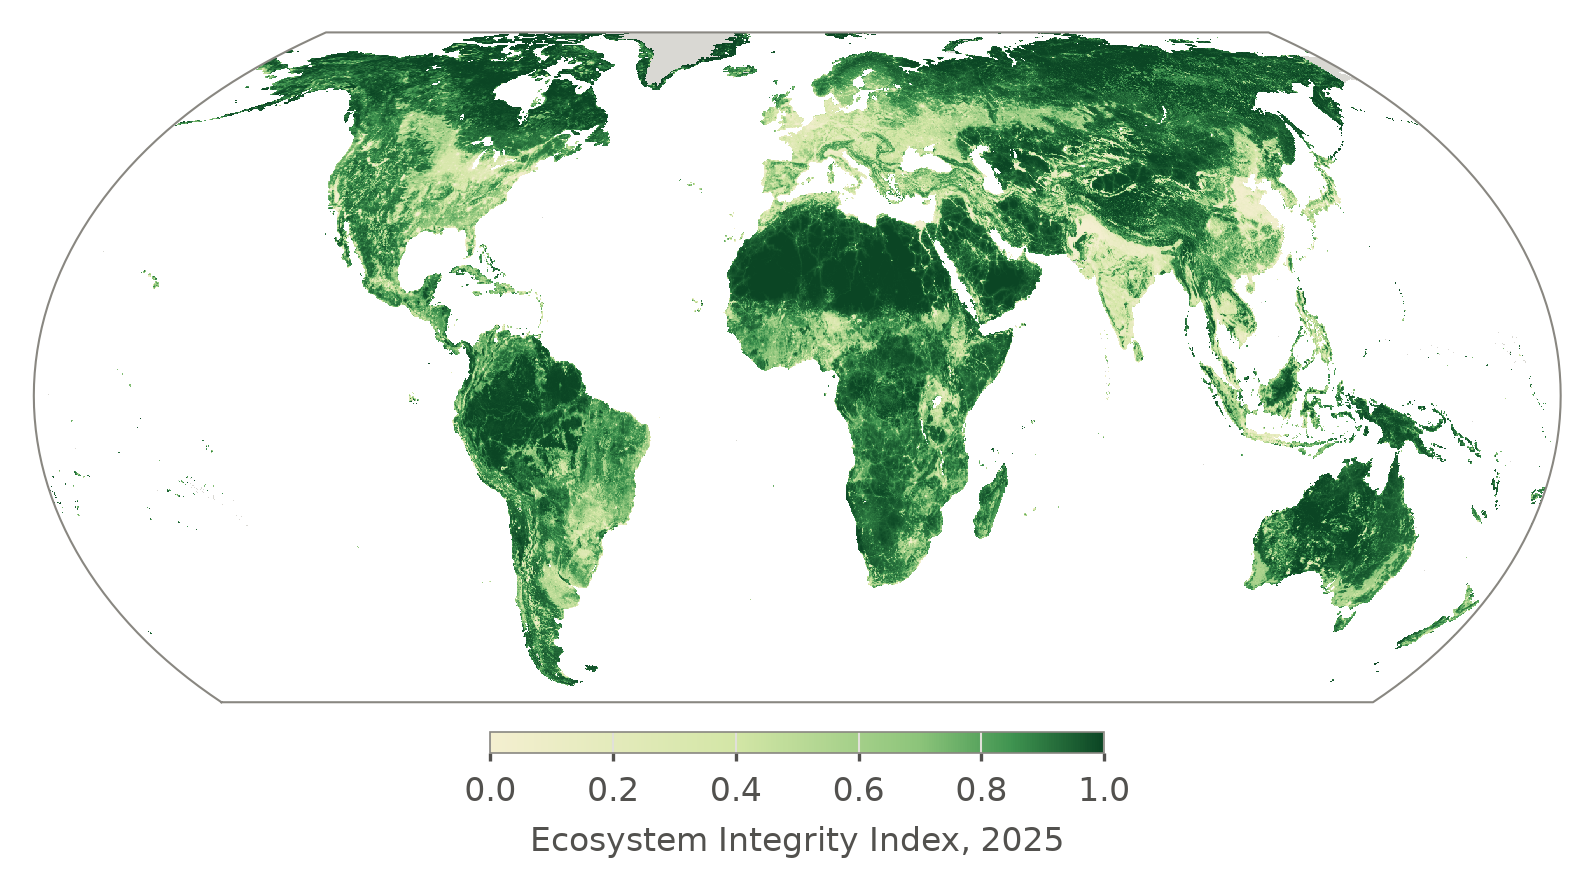
\includegraphics[width=\textwidth]{figures/eii_map_2025.png}
\caption{Ecosystem Integrity Index, reference year 2025, aggregated from 300\,m to $0.05^\circ$
by the mean of valid pixels and shown in the Equal Earth projection. Grey: land with
structural integrity but without an EII value (mostly ice and land without a potential NPP).
The maps cover $60^\circ$\,S to $80^\circ$\,N.}
\label{fig:map}
\end{figure}

Figure~\ref{fig:landcover} breaks the same sample down by the dominant ESA WorldCover 2021 class
of each point's 300\,m pixel. Tree cover, shrubland and grassland have a median EII of 0.91--0.92,
bare and sparse vegetation 0.97. Cropland has a median EII of 0.41 and built-up land 0.01,
almost entirely through structural and compositional integrity (cropland medians 0.45 and 0.54).
Functional integrity has a median of 1.00 in every class except built-up land (0.79); its
10th percentile is 0.70 on cropland and 0.84--0.93 on tree cover, shrubland and grassland. This
is the behaviour intended by the tolerance of the state score
(Section~\ref{sec:functional}): $F$ responds to strong departures from the potential and to
recent loss, while long-standing conversion is carried by $S$ and $C$. At the same points,
composition limits the EII on 53\,\%, structure on 35\,\% and function on 12\,\%.

\begin{figure}[H]
\centering
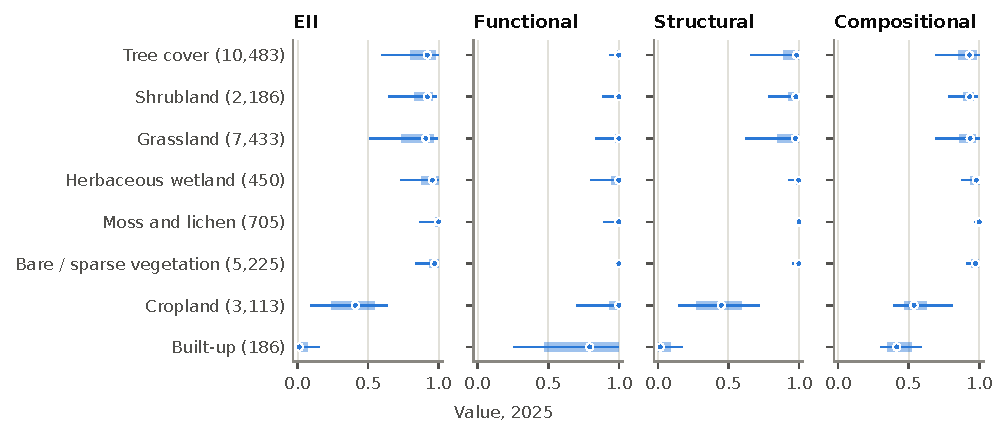
\includegraphics[width=\textwidth]{figures/eii_by_landcover_2025.pdf}
\caption{EII and its components in 2025 by the dominant ESA WorldCover 2021 class of the 300\,m
pixel, at 30,005 equal-area random land points (number per class in brackets; permanent water and classes with fewer
than 100 points omitted). Dot: median; thick bar: 25th--75th percentile; thin line:
10th--90th percentile.}
\label{fig:landcover}
\end{figure}

%==========================================================================================
\section{Validation}
\label{sec:validation}
%==========================================================================================

Ecosystem integrity is not measured in the field at global scale, so there is no direct ground
truth. Validation checks four things separately:
\begin{enumerate}
\item how well the potential model predicts NPP at natural sites it has not seen
(Section~\ref{sec:skill});
\item whether functional integrity, its state score and its change term respond to known land
use and loss without flagging intact land, at selection and in the published maps
(Section~\ref{sec:fi-selection});
\item whether the change term keeps intact land intact and detects forest loss
(Section~\ref{sec:change-validation});
\item how the global index agrees with independent indicators and with the UNEP-WCMC EII
(Section~\ref{sec:global}).
\end{enumerate}

\subsection{State score on land of known state}
\label{sec:fi-selection}

\paragraph{Design.} The state-score formula and its multipliers were selected on 500,000
equal-area validation points, each represented by a $3 \times 3$ box of 300\,m pixels, with
observed windows 2022--2024 and 2018--2020. The selection used CLMS NPP v1.1 as observed input, a
preliminary potential model and $z_s = 1$ (Table~\ref{tab:zs} covers $z_s$). Land of known state:
\begin{itemize}
\item \emph{Wild land}: wild anthromes inside very-low Low Impact Areas.
\item \emph{Used land}: cropland anthromes (classes 31--34) compared with semi-natural woodland
anthromes (51--53) in the same biome.
\item \emph{Synthetic loss}: observed NPP of intact boxes reduced by 40\,\%.
\item \emph{Real forest loss}: boxes with more than 60\,\% stand-replacing loss in the Hansen
Global Forest Change data, against undisturbed forest boxes.
\end{itemize}

\paragraph{Criteria.} Median score on wild land of at least 0.9 in every biome; 10th percentile
on wild land of at least 0.75; within-biome Spearman correlation with the Human Influence Index
of at most $-0.2$; a lower score on cropland than on semi-natural land in every biome; the mean
difference between wild and used land (\emph{signal}); and the mean penalty $1 - F_{\text{state}}$
on wild land (\emph{false alarms}).

\begin{table}[H]
\centering\footnotesize
\caption{Selected candidates for the state score; values for the 2024 / 2020 windows. Bold: the
adopted formula.}
\label{tab:fi-candidates}
\setlength{\tabcolsep}{3pt}
\begin{tabularx}{\textwidth}{Lccccc}
\toprule
Candidate & Wild p10 $\ge 0.75$ & Spearman with HII & Cropland $<$ semi-natural & Signal & False alarms \\
\midrule
Deficit only, $k = 1$ & 7/8, 8/8 & $-0.02$ / $-0.05$ & 1/11, 0/11 & 0.010 / 0.011 & 0.022 / 0.015 \\
Deficit only, $k = 1.5$ & 7/8, 8/8 & $-0.03$ / $-0.07$ & 0/11, 0/11 & 0.007 / 0.008 & 0.008 / 0.004 \\
Two-sided, no CV, $k = 1$ & 4/8, 6/8 & $-0.01$ / $-0.05$ & 6/11, 8/11 & 0.011 / 0.044 & 0.122 / 0.076 \\
Two-sided + CV, $k = 1$ & 4/8, 7/8 & $-0.08$ / $-0.12$ & 6/11, 8/11 & 0.042 / 0.069 & 0.073 / 0.036 \\
Surplus weight 0.25, $k = 1$ & 7/8, 8/8 & $-0.09$ / $-0.13$ & 4/11, 4/11 & 0.018 / 0.026 & 0.034 / 0.020 \\
Recentred two-sided + CV, $k = 1.5$ & 7/8, 8/8 & $-0.09$ / $-0.13$ & 6/11, 8/11 & 0.055 / 0.064 & 0.030 / 0.021 \\
\textbf{Recentred, $k_d = 1.0$, $k_s = 1.5$} & \textbf{7/8, 7/8} & $\mathbf{-0.09}$ / $\mathbf{-0.13}$ & \textbf{6/11, 8/11} & \textbf{0.056 / 0.067} & \textbf{0.046 / 0.029} \\
\bottomrule
\end{tabularx}
\end{table}

\begin{table}[H]
\centering\small
\caption{Response of the adopted state score to loss at selection (CLMS NPP v1.1, preliminary
potential, $z_s = 1$; 2024 / 2020 windows). Table~\ref{tab:fi-final} gives the published product.}
\begin{tabular}{lc}
\toprule
Test & Result \\
\midrule
Median score on wild land & 1.00 in every biome \\
Synthetic 40\,\% NPP loss on intact land, share of windows flagged & 0.34 / 0.31 \\
Deficit false alarms on intact land & 3.7\,\% / 1.3\,\% \\
Forest boxes with $>60\,\%$ stand-replacing loss, share flagged & 7.7\,\% / 4.8\,\% \\
Undisturbed forest boxes flagged & 1.3\,\% / 1.0\,\% \\
\bottomrule
\end{tabular}
\end{table}

\paragraph{Findings of the selection.}
\begin{itemize}
\item Surplus carries the land-use signal: deficit-only scores separate wild from used land by
only 0.007--0.011.
\item At $k_d = 1.0$, detection of a synthetic 40\,\% loss is twice that at $k_d = 1.5$ (0.34 /
0.31 against 0.18 / 0.15), at 3.7\,\% / 1.3\,\% false alarms; detection of real forest loss rises
from 3.0\,\% / 1.5\,\% to 7.7\,\% / 4.8\,\%.
\item The state score detects a minority of real forest loss: after a clear-cut, NPP falls only
20--25\,\% for one to three years in CLMS and MODIS alike. This is the gap the change term
(Section~\ref{sec:change}) addresses.
\item Without recentring, the upward drift of the CLMS record at high latitudes makes intact
boreal forest and tundra read as degraded in late windows (false alarms 0.073 in 2024, against
0.030 recentred).
\item Alternatives not adopted: a local (100\,km) recentring raises detection of scattered loss to
about 0.5 but absorbs regional loss (0.08 / 0.06 against 0.35 / 0.32); a factor per biome and
$10^\circ$ latitude band adds nothing; MODIS as the observed input separates loss worse (AUC
0.65 / 0.57 against 0.79 / 0.74), has four times the false alarms on undisturbed forest and 84\,\%
coverage.
\item No candidate meets the Spearman and cropland criteria in every biome. The limit is the
input: annual NPP does not separate many conversions (US Corn Belt observed/potential 1.13 on
modified land and 1.12 on natural land).
\item Montane grassland fails the wild-land 10th-percentile criterion (0.29 / 0.74), because the
potential model has one of its largest out-of-fold errors in this biome.
\end{itemize}

\paragraph{The published product.} The tests were repeated on the published maps of reference
years 2021 and 2025, with the published inputs (CLMS DMP V2.0.2, the final potential model and
natural CV), $z_s = 2$, the published recentring factors and the change term
(Table~\ref{tab:fi-final}). $F_{\text{state}}$ recomputed from the sampled inputs equals the
published band at every sampled pixel. The synthetic 40\,\% loss hits a random 10\,\% of the
intact boxes ($S$ and $C \ge 0.95$ in all nine pixels in both years, $P$ above the floor); the
published recentring factors are scaled per biome by the share of intact-box NPP the damage
removes, as recentring on the damaged land would. Recent forest loss is the share of the box lost
from three years before the window to its last year (2016--2021 and 2020--2025); undisturbed
forest boxes have no loss in 2001--2025. A box is flagged when its mean score is below 0.75.

\begin{table}[H]
\centering\small
\caption{Functional integrity of the published product on land of known state, reference years
2021 / 2025. $F_{\text{state}}$ and $F = F_{\text{state}} \cdot F_{\text{change}}$ as published.}
\label{tab:fi-final}
\begin{tabular}{lcc}
\toprule
Test & $F_{\text{state}}$ & $F$ \\
\midrule
Wild land: lowest biome median & 1.00 / 1.00 & 0.99 / 0.99 \\
Wild land: biomes with 10th percentile $\ge 0.75$ & 8/8, 8/8 & 7/8, 7/8 \\
Within-biome Spearman with HII, median & $-0.10$ / $-0.09$ & $-0.05$ / $-0.09$ \\
Cropland $<$ semi-natural & 6/11, 5/11 & 7/11, 6/11 \\
Signal (wild minus used) & 0.045 / 0.044 & 0.043 / 0.044 \\
False alarms (mean penalty on wild land) & 0.029 / 0.028 & 0.035 / 0.035 \\
Synthetic 40\,\% NPP loss on intact land, share flagged & 0.37 / 0.36 & -- \\
Deficit false alarms on undamaged intact land & 3.5\,\% / 2.9\,\% & -- \\
Forest boxes with $>60\,\%$ recent loss, share flagged & 5.7\,\% / 8.8\,\% & 22.9\,\% / 30.2\,\% \\
\quad AUC against undisturbed forest & 0.66 / 0.71 & 0.90 / 0.92 \\
Forest boxes with 30--60\,\% recent loss, share flagged & 2.3\,\% / 2.5\,\% & 4.4\,\% / 7.2\,\% \\
\quad AUC against undisturbed forest & 0.61 / 0.63 & 0.73 / 0.79 \\
Undisturbed forest boxes flagged & 0.5\,\% / 0.4\,\% & 0.5\,\% / 0.4\,\% \\
\bottomrule
\end{tabular}
\end{table}

\begin{itemize}
\item The published state score behaves as at selection: synthetic-loss detection 0.37 / 0.36
(selection 0.34 / 0.31), deficit false alarms 3.5\,\% / 2.9\,\% (3.7\,\% / 1.3\,\%), and a
minority of real forest loss flagged (5.7\,\% / 8.8\,\%; at selection 7.7\,\% / 4.8\,\% on the
2024 / 2020 windows).
\item $F_{\text{state}}$ meets the wild-land 10th-percentile criterion in every biome, montane
grassland included (0.79 / 0.78). With the change term, montane grassland falls below it again
(0.67 / 0.72); the other biomes pass.
\item The Spearman and cropland criteria still fail in several biomes, as at selection.
\item The change term raises detection of real forest loss three- to four-fold
(Section~\ref{sec:change-validation}) and adds almost no flags on undisturbed forest.
\end{itemize}

\subsection{Change term at near-pristine controls}
\label{sec:change-validation}

The tolerance and $k_c$ of the change term are fitted on the 19,984 near-pristine controls
(Section~\ref{sec:change}), with criteria fixed before fitting: the 10th percentile of $F$ at the
controls at least 0.90 in every window, the lowest per-biome median at least 0.90, at most twice
the global share of controls below 0.9 in any cold or montane biome, and a flag-crossing rate
between years at most 1.5 times that of $F_{\text{state}}$. On held-out scores, Terra with Suomi
NPP passes in every window 2021--2025 (10th percentile 0.908--0.916, flag-crossing ratio 1.34),
and the NOAA-20 combinations pass in 2023--2025 (0.903--0.913, ratios 1.41 and 1.47). In the
published maps, the 10th percentile of $F$ at the controls is 0.917--0.925
(Table~\ref{tab:changeglobal}).

\paragraph{Detection of forest loss.} The fit uses controls only. Detection is tested on the
published maps with the Hansen boxes of Section~\ref{sec:fi-selection}, which the fit did not see
(Table~\ref{tab:change-hansen}). $F_{\text{change}}$ alone flags 10.7\,\% / 13.8\,\% of the
boxes with more than 60\,\% recent loss (2021 / 2025) and 0.06\,\% / 0.03\,\% of undisturbed
forest boxes. $F$ is the product of the two terms, so a box that neither term flags on its own
can still fall below 0.75: $F$ flags 22.9\,\% / 30.2\,\%, more than the two terms add up to.
Detection is highest in boreal and temperate forest and lowest in tropical forest.

\begin{table}[H]
\centering\small
\caption{Share of forest boxes flagged ($F < 0.75$) by recent stand-replacing loss in the
published maps, 2021 / 2025, and AUC against undisturbed forest boxes for $F$.}
\label{tab:change-hansen}
\setlength{\tabcolsep}{4pt}
\begin{tabular}{llcccc}
\toprule
Forest & Recent loss & $F_{\text{state}}$ & $F_{\text{change}}$ & $F$ & AUC of $F$ \\
\midrule
Tropical (1--3) & $>60\,\%$ & 4.0 / 6.2\,\% & 2.4 / 3.1\,\% & 9.4 / 15.8\,\% & 0.81 / 0.92 \\
Temperate (4, 5) & $>60\,\%$ & 10.6 / 15.0\,\% & 14.7 / 21.4\,\% & 24.3 / 36.1\,\% & 0.92 / 0.86 \\
Boreal (6) & $>60\,\%$ & 5.2 / 8.1\,\% & 13.1 / 16.1\,\% & 27.6 / 34.1\,\% & 0.94 / 0.95 \\
All & $>60\,\%$ & 5.7 / 8.8\,\% & 10.7 / 13.8\,\% & 22.9 / 30.2\,\% & 0.90 / 0.92 \\
All & 30--60\,\% & 2.3 / 2.5\,\% & 0.9 / 1.4\,\% & 4.4 / 7.2\,\% & 0.73 / 0.79 \\
All & none & 0.49 / 0.39\,\% & 0.06 / 0.03\,\% & 0.53 / 0.43\,\% & -- \\
\bottomrule
\end{tabular}
\end{table}

\subsection{The global index: design}
\label{sec:global}

The published maps of reference years 2021 and 2025 are validated with the design of the
cross-indicator validation of \citet[Appendix A2]{hill2026}, so that the results can be read next
to the values reported there. 2021 is the reference year closest to 2020, the latest year of the
WCMC EII.
\begin{itemize}
\item Grid: Eckert IV equal-area projection at 1\,km. The 300\,m bands and all independent layers
are aggregated to this grid by the mean of valid pixels.
\item Sample: 500,000 equal-area random points on land (seed 42) for correlations; every
1\,km$^2$ cell of the grid for the area summaries.
\item Statistics: Pearson $r$; Spearman $\rho$ as a robustness check. All $p$-values are below
$10^{-30}$ and are not reported. No pass or fail thresholds are applied.
\item Indicators of the Kunming-Montreal framework: human footprint, Biodiversity Habitat Index
(BHI v2, 2015) for habitat and for species, and Mean Species Abundance (GLOBIO4, 2015;
\citealp{schipper2020}). The WCS Human Influence Index 2013 stands in for the
\citet{williams2020} human footprint, with the class thresholds applied on its scale.
\item Human-influence classes of \citet[Table A10]{hill2026} from anthromes \citep{ellis2010},
the human footprint and Low Impact Areas \citep{jacobson2019}, and the three
global conditions of \citet{locke2019}, derived from the human footprint and the Copernicus
LC100 2015 cropland and built-up cover.
\item Ecoregion means against the ecoregion intactness of \citet{beyer2020}.
\item For the components: nature's contributions to people \citep{chaplinkramer2019}, soil
organic carbon (GSOCmap) and the defaunation index of \citet{benitezlopez2019}, whose layer
is used as retained fauna (high values intact).
\item Comparison with the published WCMC EII 2020 raster on the WCMC grid (EPSG:4326, about
1\,km), weighted by cell area ($\cos\varphi$), on every cell where both products have a value
(97\,\% of the land that either covers).
\end{itemize}
The pairwise correlations among the four indicators on the sample lie within 0.03 of the values
reported by \citet{hill2026}, so the sample reproduces their design.

\paragraph{Pressure indicators cannot choose the functional formula.} An index built from
structure and composition alone agrees best with the four indicators, because the indicators are
themselves pressure maps; functional integrity can only lower the EII where they see no pressure.
Agreement with them is therefore a check, not the selection criterion for $F$.

\subsection{Agreement with biodiversity indicators}
\label{sec:indicators}

Table~\ref{tab:indicators} gives the correlation of the EII with the four indicators on the
446,256 sample points valid in every layer. The EII follows the human footprint closely and
agrees with BHI and MSA about as well as the published WCMC raster does. Spearman $\rho$ gives
the same picture (EII 2021: $-0.73$, 0.69, 0.69, 0.57; WCMC EII 2020: $-0.52$, 0.60, 0.60,
0.54). The values \citet{hill2026} report for their index are higher than those of their
published raster on the same points; the published raster is the reference used here.

\begin{table}[H]
\centering\small
\caption{Pearson $r$ of the EII with four biodiversity indicators, 446,256 equal-area points
valid in all layers. Last column: mean of $|r|$ over the four indicators.}
\label{tab:indicators}
\begin{tabular}{lccccc}
\toprule
 & Human footprint & BHI habitat & BHI species & MSA & Mean $|r|$ \\
\midrule
EII v2, 2021 & $-0.77$ & 0.58 & 0.60 & 0.50 & 0.613 \\
EII v2, 2025 & $-0.77$ & 0.58 & 0.61 & 0.50 & 0.615 \\
WCMC EII 2020, published raster & $-0.50$ & 0.54 & 0.55 & 0.50 & 0.524 \\
\citet{hill2026}, reported & $-0.79$ & 0.75 & 0.76 & 0.66 & 0.740 \\
\bottomrule
\end{tabular}
\end{table}

Ecoregion means of the EII against the ecoregion intactness of \citet{beyer2020}, over the 789
ecoregions with at least 100\,km$^2$ of valid cells, give Pearson $r = 0.51$ and Spearman
$\rho = 0.80$ for 2021 (2025: 0.51 and 0.81). The WCMC EII 2020 reaches 0.41 and 0.56 on 796
ecoregions; \citet{hill2026} report $r = 0.84$ for their index.

\subsection{Separation of human-influence classes}
\label{sec:classes}

For each classification, the AUC is the probability that a random km$^2$ of the
least-influenced class scores higher than one of the most-influenced class (0.5: no separation;
1: complete separation), computed over the full 1\,km grid (Table~\ref{tab:auc},
Figure~\ref{fig:influence}). The EII separates heavily used from wild land more sharply than the
WCMC EII under all four classifications. Structural integrity alone separates the classes
slightly better than the EII: the classifications are built from the same kind of land-use
information, while functional and compositional integrity can lower the EII on land these maps
class as wild. Under the conditions of \citet{locke2019}, mean EII in 2021 is 0.94 in large wild
areas, 0.77 in shared lands and 0.34 in cities and farms.

\begin{table}[H]
\centering\small
\caption{Separation of the least- from the most-influenced class (AUC), full Eckert IV 1\,km
grid.}
\label{tab:auc}
\begin{tabular}{lcccc}
\toprule
Classification (least vs most influenced) & EII 2021 & EII 2025 & $S$ 2021 & WCMC EII 2020 \\
\midrule
Anthromes (wild vs used) & 0.905 & 0.901 & 0.917 & 0.898 \\
Human footprint ($0$ vs $>3$) & 0.881 & 0.885 & 0.921 & 0.781 \\
Low Impact Areas (very low impact vs outside) & 0.902 & 0.906 & 0.929 & 0.832 \\
Locke et al.\ (large wild areas vs cities and farms) & 0.989 & 0.989 & 0.999 & 0.887 \\
\bottomrule
\end{tabular}
\end{table}

\begin{figure}[H]
\centering
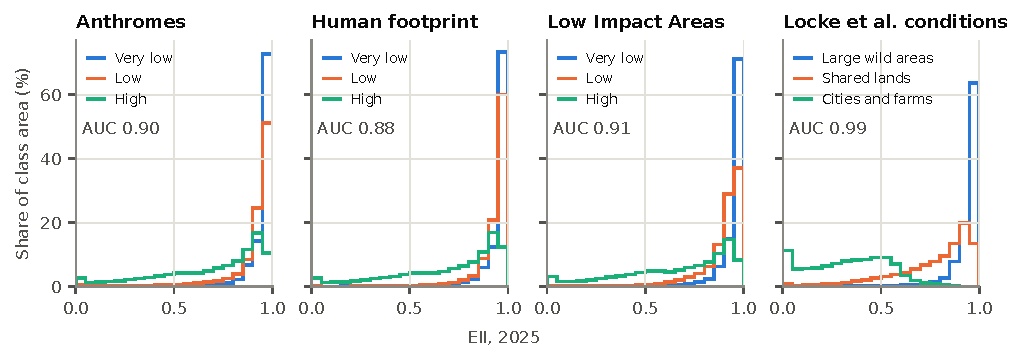
\includegraphics[width=\textwidth]{figures/eii_by_influence_class_2025.pdf}
\caption{Distribution of the EII 2025 over the human-influence classes of four classifications,
as the share of each class's area per 0.05 bin of EII (full Eckert IV 1\,km grid). Anthromes,
human footprint and Low Impact Areas: very low, low and high influence (Table A10 of
\citealp{hill2026}); Locke et al.: the three global conditions. AUC: very low influence (large
wild areas) against high influence (cities and farms).}
\label{fig:influence}
\end{figure}

\subsection{Components}
\label{sec:components-validation}

Structural and compositional integrity are strongly correlated, because both are derived from
maps of human pressure; functional integrity is nearly independent of both
(Table~\ref{tab:components}). Functional integrity limits the EII on about one sixth of the
sample points, mostly on otherwise intact land, so it carries information the other two
components do not. The index therefore carries two largely independent signals, pressure and
productivity, rather than three.

\begin{table}[H]
\centering\small
\caption{Correlation between the components (Pearson $r$) and share of sample points limited by
each component, 500,000-point equal-area sample on the 1\,km grid.}
\label{tab:components}
\begin{tabular}{lccc}
\toprule
 & 2021 & 2025 & \citet{hill2026} \\
\midrule
$S$ with $C$ & 0.90 & 0.89 & 0.54 \\
$S$ with $F$ & 0.19 & 0.19 & 0.10 \\
$C$ with $F$ & 0.18 & 0.19 & 0.09 \\
Limited by $C$ / $S$ / $F$ & 52 / 32 / 16\,\% & 53 / 31 / 16\,\% & \\
\bottomrule
\end{tabular}
\end{table}

Compositional integrity agrees with the biodiversity layers more closely than \citet{hill2026}
report for their compositional component (Table~\ref{tab:component-layers}). Functional integrity shows no
relationship with nature's contributions to people or with soil organic carbon, as in
\citet{hill2026}. These layers measure how much of a service is supplied, not whether the land
functions as it would without human pressure, so a weak relationship is expected.

\begin{table}[H]
\centering\small
\caption{Pearson $r$ of the compositional and functional components with independent layers,
2021, and the values reported by \citet{hill2026}.}
\label{tab:component-layers}
\begin{tabular}{llrcc}
\toprule
Component & Layer & Points & $r$ & \citet{hill2026} \\
\midrule
Compositional & BHI species & 492,175 & 0.66 & 0.52 \\
 & BHI habitat & 492,175 & 0.63 & -- \\
 & MSA & 493,986 & 0.56 & 0.44 \\
 & Retained fauna (tropics) & 112,722 & 0.55 & 0.23 \\
Functional & Pollination & 243,348 & $-0.10$ & $-0.01$ \\
 & Nutrient retention & 398,215 & $-0.08$ & $-0.06$ \\
 & Nitrogen retention & 397,913 & $-0.06$ & 0.01 \\
 & Nutrient delivery ratio & 397,923 & $-0.06$ & -- \\
 & Soil organic carbon (GSOCmap) & 457,249 & 0.05 & 0.01 \\
\bottomrule
\end{tabular}
\end{table}

\subsection{Comparison with the WCMC EII}
\label{sec:wcmc}

Table~\ref{tab:wcmc} compares the EII with the published WCMC EII 2020 on every shared cell of
the WCMC grid. Both products agree on wild land: the densest part of their joint distribution lies near
(1,\,1). The
differences are regional and systematic (Table~\ref{tab:wcmc-biome}). The EII is higher on
drylands and rangelands (Australia, the Sahel, southern Africa, the Central Asian steppe, the
western United States, Patagonia) and in the Arctic tundra; the WCMC EII places large areas of
rangeland at 0.40--0.46. The EII is lower in the farmed and settled temperate broadleaf
regions (Europe, the eastern United States, eastern China) and in India, where its structural
component scores cropland and settlements lower. Agreement is high in forest biomes with a
clear gradient from intact to converted land ($r$ 0.78--0.90) and low in grassland, savanna,
tundra and desert, where the two products judge grazing land and sparse vegetation differently.

\begin{table}[H]
\centering\small
\caption{Agreement of the EII with the WCMC EII 2020 on the shared cells of the WCMC grid,
area-weighted. Spearman $\rho$ on the equal-area sample (447,577 and 447,661 of 500,000 points
valid for 2021 and 2025).}
\label{tab:wcmc}
\begin{tabular}{lcc}
\toprule
Measure & EII 2021 & EII 2025 \\
\midrule
Pearson $r$ & 0.529 & 0.527 \\
Spearman $\rho$ & 0.592 & 0.579 \\
Mean EII (WCMC EII 2020: 0.763) & 0.805 & 0.804 \\
Mean difference, EII minus WCMC & $+0.042$ & $+0.041$ \\
Mean absolute difference & 0.154 & 0.155 \\
Root-mean-square difference & 0.235 & 0.235 \\
1st / 99th percentile of the difference & $-0.48$ / $+0.59$ & $-0.48$ / $+0.59$ \\
Share of area differing by more than 0.2 & 29\,\% & 29\,\% \\
\bottomrule
\end{tabular}
\end{table}

\begin{table}[H]
\centering\small
\caption{Mean EII 2021 and WCMC EII 2020 per biome on the shared cells, area-weighted, with the
mean difference (EII minus WCMC), the mean absolute difference and the area-weighted Pearson $r$
across cells.}
\label{tab:wcmc-biome}
\begin{tabular}{lccccc}
\toprule
Biome & WCMC 2020 & EII 2021 & Difference & Mean abs.\ diff. & $r$ \\
\midrule
Tropical moist broadleaf & 0.841 & 0.796 & $-0.046$ & 0.082 & 0.88 \\
Tropical dry broadleaf & 0.714 & 0.658 & $-0.055$ & 0.115 & 0.86 \\
Tropical conifer & 0.791 & 0.815 & $+0.024$ & 0.136 & 0.43 \\
Temperate broadleaf & 0.688 & 0.587 & $-0.101$ & 0.134 & 0.90 \\
Temperate conifer & 0.841 & 0.827 & $-0.014$ & 0.123 & 0.49 \\
Boreal & 0.948 & 0.932 & $-0.016$ & 0.060 & 0.49 \\
Savanna & 0.671 & 0.835 & $+0.164$ & 0.213 & 0.37 \\
Temperate grassland & 0.562 & 0.679 & $+0.117$ & 0.242 & 0.13 \\
Flooded grassland & 0.599 & 0.789 & $+0.189$ & 0.280 & 0.27 \\
Montane grassland & 0.607 & 0.814 & $+0.207$ & 0.311 & 0.07 \\
Tundra & 0.871 & 0.944 & $+0.073$ & 0.148 & 0.04 \\
Mediterranean & 0.695 & 0.644 & $-0.051$ & 0.126 & 0.78 \\
Desert and xeric & 0.800 & 0.873 & $+0.074$ & 0.171 & 0.40 \\
Mangrove & 0.762 & 0.702 & $-0.060$ & 0.122 & 0.84 \\
\bottomrule
\end{tabular}
\end{table}

Across the 415 World Terrestrial Ecosystems of \citet{sayre2020}, with each product averaged on
its own valid mask, the mean of the ecosystem means is similar (EII 2021: 0.678; WCMC EII 2020:
0.689), but the EII spreads them more widely (standard deviation 0.30 against 0.20): 59
ecosystems average 0.25 or less in the EII, 7 in the WCMC EII.

\subsection{Not validated}

\begin{itemize}
\item Plot-level accuracy: there is no global set of field measurements of integrity.
\item Functional integrity on non-forest degradation (rangeland, drought die-off), for which no
independent reference data were available.
\item Change over time: the WCMC EII ends in 2020 and the independent layers are single epochs
(2000--2015), so year-to-year changes of the EII are not compared with an external series.
\item The potential model on the smallest biomes with a full leave-biome-out test; the
leave-realm-out results stand in.
\item The comparison with the Red List of Ecosystems of South Africa (Fig.~A7 of
\citealp{hill2026}): the data could not be obtained.
\end{itemize}

%==========================================================================================
\section{Limitations and interpretation}
%==========================================================================================

\begin{description}[leftmargin=1.2em]
\item[Contemporary reference.] The potential describes natural vegetation under present
conditions. An ecosystem that matches it scores 1 even if it once produced more.
\item[Extrapolation.] In regions with a long history of intensive use, few reference sites
remain and the potential is learned partly from similar climates elsewhere; in semi-arid regions
without natural land it partly describes lightly used land.
\item[Detection limits of $F$.] Deviations inside the tolerances are not penalised.
$F_{\text{state}}$ responds to strong and lasting changes in productivity; a surplus is penalised
less steeply than a deficit, and irrigated desert agriculture still scores close to 0.
$F_{\text{change}}$ responds to vegetation loss since the 2009--2018 baseline for as long as EVI
stays below the baseline; it has no expiry and was evaluated on events up to six years old. Land converted before the baseline and kept in
the same use scores $F_{\text{change}} = 1$; $F$ is near 1 on most land by design.
\item[Ending satellite records.] The change term depends on MODIS Terra and VIIRS. Suomi NPP
ended on 2 November 2026 and Terra is planned to end around January 2027; from 2027 NOAA-20 alone
serves, with a noisier ratio. For a reference year in which no sensor has complete data for the
window, $F = F_{\text{state}}$. On 3\,\% of land, mostly deserts, no sensor has a change value.
\item[Shared response to clearing.] $F_{\text{change}}$ is not masked where forest loss is
mapped, so a recent clearing can lower both $F$ and $C$.
\item[Absorbed biome-wide change.] Recentring absorbs change uniform across a biome within one
window.
\item[Climate versus management.] $F$ does not separate productivity changes caused by climate
from those caused by land management. The change term has no biome-level recentring, and its flags
concentrate in drylands and fire regions, where much of the loss is likely drought or fire.
\item[Pressure, not habitat.] $S$ is built from human pressure. Low-pressure land that is not
natural habitat counts by its low pressure, and small natural features inside high-pressure
pixels are not seen. Unmapped degradation such as selective logging leaves $S$ high in tropical
forest. $S$ measures the amount of good land nearby, not functional connectivity. Its quality
curve is calibrated against a land-cover bound, not a measured target.
\item[Static structure.] HMI 2022 is used for every reference year; $S$ does not register change
after 2022.
\item[Modelled composition.] BII is modelled from mapped pressures and PREDICTS surveys, and can
anticipate losses or gains not yet realised on the ground.
\item[Annual change.] Year-to-year change comes from observed NPP, EVI and BII. The three-year
windows share two years between consecutive reference years, so change is damped and lagged. Small
changes in $F$ at single pixels can come from weather within the window and from the recentring
factors.
\item[Resolution.] The grid spacing is $1/336^\circ$; a pixel covers about $11\cos\varphi$\,ha
(11\,ha at the equator, 7.8\,ha at $45^\circ$). The effective resolution is coarser than the grid:
the potential rests on climate predictors at about 1\,km, the change term on 250--500\,m MODIS
and VIIRS EVI, and structural integrity on an exponential neighbourhood (5\,km scale, truncated at 26.5\,km). Mixed pixels occur
at sharp boundaries. Single 300\,m pixels should not be interpreted on their own; aggregates over
properties, management units or regions are more robust.
\end{description}

%==========================================================================================
\section*{Data and code availability}
%==========================================================================================

The EII v2 maps, the potential-NPP maps and the training tables are published under the Creative
Commons Attribution 4.0 licence (CC BY 4.0), attribution: The Landbanking Group. They are
available as
\begin{itemize}
\item cloud-optimised GeoTIFFs in the requester-pays bucket
\nolinkurl{gs://landler-opendata-gee-assets/products/eii/v2_0/}, and
\item the Earth Engine collection
\nolinkurl{projects/landler-open-data/assets/products/eii/v2_0/release/global}.
\end{itemize}
The third-party
inputs keep their own licence and attribution terms (Table~\ref{tab:inputs} and the online
documentation). The code of the calculation, the training, the production run and the validation
is released under the Apache License 2.0 at
\url{https://github.com/landler-io/ecosystem-integrity-index}.

%==========================================================================================
\begin{thebibliography}{99}
\setlength{\itemsep}{2pt}
\small

\bibitem[Amatulli et~al.(2020)]{amatulli2020}
Amatulli, G., McInerney, D., Sethi, T., Strobl, P., \& Domisch, S. (2020). Geomorpho90m,
empirical evaluation and accuracy assessment of global high-resolution geomorphometric layers.
\emph{Scientific Data}, 7, 162.

\bibitem[Andr\'en(1994)]{andren1994}
Andr\'en, H. (1994). Effects of habitat fragmentation on birds and mammals in landscapes with
different proportions of suitable habitat: a review. \emph{Oikos}, 71, 355--366.

\bibitem[Ben\'itez-L\'opez et~al.(2019)]{benitezlopez2019}
Ben\'itez-L\'opez, A., et~al. (2019). Intact but empty forests? Patterns of hunting-induced
mammal defaunation in the tropics. \emph{PLoS Biology}, 17, e3000247.

\bibitem[Beyer et~al.(2020)]{beyer2020}
Beyer, H.~L., Venter, O., Grantham, H.~S., \& Watson, J.~E.~M. (2020). Substantial losses in
ecoregion intactness highlight urgency of globally coordinated action. \emph{Conservation
Letters}, 13, e12692.

\bibitem[Chaplin-Kramer et~al.(2019)]{chaplinkramer2019}
Chaplin-Kramer, R., et~al. (2019). Global modeling of nature's contributions to people.
\emph{Science}, 366, 255--258.

\bibitem[Dinerstein et~al.(2017)]{dinerstein2017}
Dinerstein, E., et~al. (2017). An ecoregion-based approach to protecting half the terrestrial
realm. \emph{BioScience}, 67, 534--545.

\bibitem[Ellis et~al.(2010)]{ellis2010}
Ellis, E.~C., Klein Goldewijk, K., Siebert, S., Lightman, D., \& Ramankutty, N. (2010).
Anthropogenic transformation of the biomes, 1700 to 2000. \emph{Global Ecology and
Biogeography}, 19, 589--606.

\bibitem[Fahrig(2003)]{fahrig2003}
Fahrig, L. (2003). Effects of habitat fragmentation on biodiversity. \emph{Annual Review of
Ecology, Evolution, and Systematics}, 34, 487--515.

\bibitem[Gassert et~al.(2026)]{gassert2026}
Gassert, F., Mazzarello, J., \& Hyde, S. (2026). \emph{Biodiversity Intactness v1.1}. Impact
Observatory and Vizzuality.

\bibitem[Hansen et~al.(2013)]{hansen2013}
Hansen, M.~C., et~al. (2013). High-resolution global maps of 21st-century forest cover change.
\emph{Science}, 342, 850--853.

\bibitem[Hart-Davis et~al.(2021)]{hartdavis2021}
Hart-Davis, M.~G., et~al. (2021). EOT20: a global ocean tide model from multi-mission satellite
altimetry. \emph{Earth System Science Data}, 13, 3869--3884.

\bibitem[Hill et~al.(2026)]{hill2026}
Hill, S.~L.~L., et~al. (2026). The ecosystem integrity index: a component indicator in the
Kunming-Montreal global biodiversity framework reveals the integrity of terrestrial ecosystems
globally. \emph{Ecological Indicators}, 190, 115314.

\bibitem[Hudson et~al.(2017)]{hudson2017}
Hudson, L.~N., et~al. (2017). The database of the PREDICTS (Projecting Responses of Ecological
Diversity In Changing Terrestrial Systems) project. \emph{Ecology and Evolution}, 7, 145--188.

\bibitem[Jacobson et~al.(2019)]{jacobson2019}
Jacobson, A.~P., Riggio, J., Tait, A.~M., \& Baillie, J.~E.~M. (2019). Global areas of low
human impact (`Low Impact Areas') and fragmentation of the natural world. \emph{Scientific
Reports}, 9, 14179.

\bibitem[Karger et~al.(2017)]{karger2017}
Karger, D.~N., et~al. (2017). Climatologies at high resolution for the earth's land surface
areas. \emph{Scientific Data}, 4, 170122.

\bibitem[Kennedy et~al.(2019)]{kennedy2019}
Kennedy, C.~M., Oakleaf, J.~R., Theobald, D.~M., Baruch-Mordo, S., \& Kiesecker, J. (2019).
Managing the middle: a shift in conservation priorities based on the global human modification
gradient. \emph{Global Change Biology}, 25, 811--826.

\bibitem[Lehner et~al.(2025)]{lehner2025}
Lehner, B., et~al. (2025). The Global Lakes and Wetlands Database (GLWD) version 2. \emph{Earth
System Science Data}, 17, 2277--2329.

\bibitem[Lei et~al.(2018)]{lei2018}
Lei, J., G'Sell, M., Rinaldo, A., Tibshirani, R.~J., \& Wasserman, L. (2018). Distribution-free
predictive inference for regression. \emph{Journal of the American Statistical Association},
113, 1094--1111.

\bibitem[Locke et~al.(2019)]{locke2019}
Locke, H., et~al. (2019). Three global conditions for biodiversity conservation and sustainable
use: an implementation framework. \emph{National Science Review}, 6, 1080--1082.

\bibitem[Meinshausen(2006)]{meinshausen2006}
Meinshausen, N. (2006). Quantile regression forests. \emph{Journal of Machine Learning
Research}, 7, 983--999.

\bibitem[Newbold et~al.(2016)]{newbold2016}
Newbold, T., et~al. (2016). Has land use pushed terrestrial biodiversity beyond the planetary
boundary? A global assessment. \emph{Science}, 353, 288--291.

\bibitem[Sayre et~al.(2020)]{sayre2020}
Sayre, R., et~al. (2020). An assessment of the representation of ecosystems in global protected
areas using new maps of World Climate Regions and World Ecosystems. \emph{Global Ecology and
Conservation}, 21, e00860.

\bibitem[Schipper et~al.(2020)]{schipper2020}
Schipper, A.~M., et~al. (2020). Projecting terrestrial biodiversity intactness with GLOBIO 4.
\emph{Global Change Biology}, 26, 760--771.

\bibitem[Scholes \& Biggs(2005)]{scholes2005}
Scholes, R.~J., \& Biggs, R. (2005). A biodiversity intactness index. \emph{Nature}, 434,
45--49.

\bibitem[Theobald et~al.(2020)]{theobald2020}
Theobald, D.~M., et~al. (2020). Earth transformed: detailed mapping of global human
modification from 1990 to 2017. \emph{Earth System Science Data}, 12, 1953--1972.

\bibitem[Theobald(2024a)]{theobald2024ts}
Theobald, D.~M. (2024a). Global human modification datasets of terrestrial ecosystems from 1990
to 2020. Zenodo, doi:10.5281/zenodo.14449495.

\bibitem[Theobald(2024b)]{theobald2024}
Theobald, D.~M. (2024b). Global human modification datasets of terrestrial ecosystems for 2022.
Zenodo, doi:10.5281/zenodo.14502573.

\bibitem[Vovk et~al.(2005)]{vovk2005}
Vovk, V., Gammerman, A., \& Shafer, G. (2005). \emph{Algorithmic Learning in a Random World}.
Springer.

\bibitem[Williams et~al.(2020)]{williams2020}
Williams, B.~A., et~al. (2020). Change in terrestrial human footprint drives continued loss of
intact ecosystems. \emph{One Earth}, 3, 371--382.

\bibitem[Yamazaki et~al.(2017)]{yamazaki2017}
Yamazaki, D., et~al. (2017). A high-accuracy map of global terrain elevations.
\emph{Geophysical Research Letters}, 44, 5844--5853.

\end{thebibliography}

\end{document}
